% Template:     Tesis LaTeX
% Documento:    Archivo principal
% Versión:      3.4.2 (07/02/2025)
% Codificación: UTF-8
%
% Autor: Pablo Pizarro R.
%        pablo@ppizarror.com
%
% Manual template: [https://latex.ppizarror.com/tesis]
% Licencia MIT:    [https://opensource.org/licenses/MIT]

% CREACIÓN DEL DOCUMENTO
\documentclass[
	spanish, % Idioma: spanish, english, etc.	
	letterpaper, oneside
]{book}

% INFORMACIÓN DEL DOCUMENTO
\def\documenttitle {Implementación de Algoritmos de Reconocimiento de Objetos para la Identificación de Fallas en Correas Transportadoras}
\def\documentsubtitle {}
\def\degreetitle {
Informe de Avance Memoria de Título
}

\def\universityname {Universidad de Chile}
\def\universityfaculty {Facultad de Ciencias Físicas y Matemáticas}
\def\universitydepartment {Departamento de Ingeniería Mecánica}
\def\universitydepartmentimage {departamentos/uchile2}
\def\universitydepartmentimagecfg {height=3cm}
\def\universitylocation {Santiago de Chile}

% INTEGRANTES, PROFESORES Y FECHAS
\def\documentauthor {FERNANDO IGNACIO NAVARRETE URRUTIA}
\def\documentdate {\the\year}

\def\portrait {
	\begin{center}
	\vspace{1.5cm} ~ \\
	\MakeUppercase{\textbf{\documenttitle}} ~ \\
	\vspace{1.5cm}
	\MakeUppercase{\degreetitle} ~ \\
    \vspace{1.5cm}
	\begin{tabular}{c}\MakeUppercase{\textbf{\documentauthor}} \\ \\
		\vspace{1.0cm} \\
		PROFESOR GUÍA: \\
		VIVIANA MERUANE NARANJO \\
		\vspace{0.5cm} \\
        PROFESOR CO-GUÍA: \\
        HAROLD VALENZUELA COLOMA\\
        \vspace{0.5cm} \\
		% COMISIÓN: \\
		% PROFESOR 2 \\
		% PROFESOR 3 \\
		% \vspace{0.5cm} \\
		% Este trabajo ha sido parcialmente financiado por: \\
		% NOMBRE INSTITUCIÓN \\
		% \vspace{0.5cm} \\
		\MakeUppercase{\universitylocation} \\
		\MakeUppercase{\documentdate}
	\end{tabular}
	\end{center}
}
\def\abstracttable {
	\begin{tabular}{l}
		RESUMEN EJECUTIVO DEL INFORME FINAL \\ PARA OPTAR AL TÍTULO DE \\ INGENIERO CIVIL MECÁNICO \\
        POR: \MakeUppercase{\documentauthor} \\
		FECHA: \MakeUppercase{\documentdate} \\
		PROF. GUÍA: VIVIANA MERUANE NARANJO \\
        PROF. CO-GUÍA: HAROLD VALENZUELA COLOMA
	\end{tabular}
}

% IMPORTACIÓN DEL TEMPLATE
\input{template}

% INICIO DE LAS PÁGINAS
\begin{document}

% PORTADA
\templatePortrait

% CONFIGURACIÓN DE PÁGINA Y ENCABEZADOS
\templatePagecfg

% RESUMEN O ABSTRACT
\begin{abstractd}
	La detección temprana de fallas en correas transportadoras es fundamental para evitar paradas no programadas y pérdidas operativas en industrias críticas. Los métodos tradicionales basados en inspección visual presentan limitaciones en velocidad, costo y precisión. En contraste, las técnicas de aprendizaje profundo, especialmente aquellas basadas en redes neuronales convolucionales (CNN) y arquitecturas \textit{Transformer}, ofrecen soluciones automatizadas y escalables para la clasificación de fallas mediante visión computacional, favoreciendo el mantenimiento predictivo y la supervisión continua.\\

Este trabajo de memoria de título se enfoca en implementar modelos de detección de fallas en correas transportadoras mediante técnicas de visión computacional y aprendizaje profundo. El objetivo general es implementar y evaluar algoritmos de detección de objetos basados en inteligencia artificial. Entre los objetivos específicos destacan la implementación y entrenamiento con bases de datos etiquetadas, la programación de modelos basados en CNN (YOLO y SSD) y modelos \textit{Transformer} (DETR y DINO). Por último, se realiza una evaluación comparativa mediante métricas estándar de visión por computadora.\\

La metodología contempla la implementación y el entrenamiento de modelos en entornos de cómputo especializados, utilizando bases de datos segmentadas rigurosamente en entrenamiento, validación y prueba. Los resultados posicionan al modelo YOLOv5 como la arquitectura más eficiente y de mayor viabilidad industrial, superando a SSD512 y a los modelos de atención global. Si bien los detectores basados en \textit{Transformers} demostraron ventajas teóricas al aislar defectos complejos como perforaciones, su desempeño general se vio penalizado por la escala reducida de los datos y las restricciones de capacidad física (\textit{hardware}). A partir de estos hallazgos, se propone como trabajo futuro la exploración de arquitecturas híbridas y una optimización de hiperparámetros. Para garantizar la reproducibilidad, la estructura de trabajo, registros de métricas y detalles se encuentran almacenados en un repositorio de código abierto (\href{https://github.com/FernandoN23/Implementation-of-Object-Detection-for-Conveyor-Belt-Defect-Detection}{\textit{Implementation of Object Detection for Conveyor Belt Defect Detection}}).
\end{abstractd}

% % DEDICATORIA / AGRADECIMIENTOS
% \begin{dedicatory}
% 	A mi querido gato, \\ que no hace nada por nadie, \\ pero incluso así, \\ se ganó un espacio en esta sección. 
% \end{dedicatory}

% % AGRADECIMIENTOS
% \begin{acknowledgments}
% 	\lipsum[1]
% \end{acknowledgments}

% TABLA DE CONTENIDOS - ÍNDICE
\templateIndex

% CONFIGURACIONES FINALES
\templateFinalcfg

% ======================= INICIO DEL DOCUMENTO =======================

\counterwithin{figure}{section}
\counterwithin{table}{section}
\counterwithin{equation}{section}
\chapter{Introducción}

Las correas transportadoras constituyen un componente crítico en la minería y en diversas industrias intensivas en el transporte de materiales a granel, al permitir el movimiento continuo y eficiente de grandes volúmenes de carga sobre largas distancias. Su operación sostenida se encuentra estrechamente vinculada a la productividad global de la planta, de modo que fallas inesperadas en la correa o en sus componentes asociados se traducen directamente en detenciones no programadas, sobrecostos de mantenimiento y potenciales riesgos para la seguridad de las personas y equipos. En este contexto, asegurar la disponibilidad y confiabilidad de las correas transportadoras es un requisito fundamental para la operación industrial moderna. \\

Durante su vida útil, las correas están expuestas a condiciones de servicio severas que favorecen la aparición de diversos modos de daño, tales como desgaste abrasivo, grietas o rasgaduras, roturas de empalme y fallas asociadas a desalineamientos prolongados. Estos defectos pueden evolucionar desde deterioros superficiales hasta fallas catastróficas, comprometiendo la integridad estructural de la correa y de la línea de transporte \cite{khanna2022types}. La gran longitud de los sistemas transportadores y la variabilidad de las condiciones ambientales dificultan su inspección exhaustiva, incrementando la probabilidad de que daños incipientes no sean detectados oportunamente. \\

Tradicionalmente, el monitoreo del estado de las correas transportadoras se ha basado en rondas de inspección visual realizadas por personal especializado, apoyadas ocasionalmente por dispositivos de medición puntual. Si bien este enfoque ha sido la práctica estándar en la industria, presenta limitaciones importantes: la cobertura espacial y temporal de las inspecciones es restringida, la detección de fallas depende fuertemente de la experiencia del inspector y, en muchos casos, es necesario detener o intervenir la correa para realizar revisiones detalladas, afectando la continuidad operacional. Estas restricciones han motivado el desarrollo de estrategias de monitoreo automatizado que reduzcan la carga operativa y mejoren la detección temprana de daños \cite{angulo2024deteccion}. \\

En paralelo, los avances en visión computacional y aprendizaje profundo (\textit{Deep Learning}) han permitido desarrollar modelos capaces de identificar y localizar objetos o patrones específicos directamente a partir de imágenes, sin requerir una etapa manual de ingeniería de características. En particular, los detectores de una sola etapa (\textit{one-stage detectors}), como las familias YOLO y SSD, han mostrado un compromiso favorable entre precisión y velocidad de inferencia en escenarios de detección en tiempo casi real, lo que los convierte en candidatos naturales para su aplicación en el monitoreo continuo de correas transportadoras \cite{zhang2021deep,zhang2021one_stage}. Adicionalmente, trabajos recientes han demostrado la viabilidad de utilizar arquitecturas basadas en YOLO para la detección de fallas o condiciones anómalas en sistemas transportadores, reforzando el potencial de estas técnicas en entornos industriales \cite{angulo2024deteccion}. \\

Considerando este contexto, la presente memoria aborda el problema de la identificación automática de fallas en correas transportadoras mediante modelos de detección de objetos basados en aprendizaje profundo, abarcando tanto detectores de una sola etapa como arquitecturas recientes basadas en \textit{transformers}. El trabajo se centra en la implementación, entrenamiento y evaluación comparativa de estos enfoques sobre un conjunto de datos específico de defectos en correas, con el objetivo de analizar su capacidad para detectar distintos tipos de daño y su adecuación para ser integrados en sistemas de monitoreo y mantenimiento predictivo en un entorno cercano al operativo, según la eficiencia y exigencia de cada modelo. \\





%%%%%%%%%%%%%%%%%%%%%%%%%%%%%%%%%%%%%%%%%%%%
\section{Objetivo General}

Implementar y evaluar algoritmos
de detección de objetos, basados en
inteligencia artificial, para la identificación automática de
fallas en correas transportadoras.



\section{Objetivos Específicos}


Para lograr el objetivo general en este futuro trabajo de memoria de título, se propone cumplir con los siguientes
objetivos específicos:

\begin{enumerate}
    \item Implementar modelos de detección de objetos basados en redes convolucionales, tales como YOLO (You Only Look Once) y sus variantes, y SSD (Single Shot Multibox Detector).

    \item Implementar modelos de detección de objetos basados en redes neuronales con arquitectura tipo transformer, tales como DETR (DEtection TRansformer) y DINO.

    \item Entrenar algoritmos de detección de objetos utilizando bases de datos con registros de fallas en correas transportadoras.

    \item Comparar el desempeño de los modelos en la detección de distintos tipos de fallas mediante el uso de métricas de evaluación cuantitativas.

    
\end{enumerate}


\section{Alcances}

\begin{itemize}
    \item El entrenamiento de los algoritmos de detección se realizará exclusivamente con bases de datos públicas disponibles en la web que contengan registros de fallas en correas transportadoras.

    \item Considerar el uso de datos sin etiquetar, los cuales serán procesados mediante estrategias de etiquetado manual o mediante técnicas no supervisadas y/o auto-supervisadas, según su aplicabilidad.

    \item Evaluar el rendimiento de los modelos seleccionados (YOLO, SSD, DETR y DINO) en la detección y clasificación de fallas, utilizando una misma base de datos con partición en conjuntos de entrenamiento, validación y prueba. Posteriormente se evaluarán utilizando métricas estándar de evaluación.
    
\end{itemize}
\chapter{Antecedentes}

\section{Estado del arte en la identificación de fallas en correas transportadoras}

\par El aprendizaje profundo (\textit{Deep Learning}) surge como una evolución de los enfoques clásicos de aprendizaje automático (\textit{Machine Learning}), al introducir redes neuronales profundas capaces de aprender de forma automática representaciones jerárquicas directamente desde los datos. En los métodos tradicionales de \textit{Machine Learning}, la etapa de ingeniería de características recae en el especialista, quien define manualmente descriptores (por ejemplo, basados en bordes, texturas o histogramas) y luego entrena un clasificador independiente sobre dichas representaciones. En contraste, en \textit{Deep Learning} la misma red realiza de manera integrada la extracción de características y la decisión final, aprendiendo dichas representaciones de alto nivel a partir de grandes volúmenes de datos. Esto ha permitido superar de forma sistemática a los métodos convencionales en tareas de clasificación, segmentación y detección de objetos. Adicionalmente, el aprendizaje por transferencia (\textit{transfer learning}) ha cobrado relevancia en escenarios con escasez de datos etiquetados, al reutilizar modelos profundos preentrenados en bases de datos extensas y ajustarlos a nuevas tareas de visión por computador, mejorando el rendimiento y reduciendo el costo computacional del entrenamiento \cite{gupta2022deep}.\\

\begin{figure}[H]
    \centering
    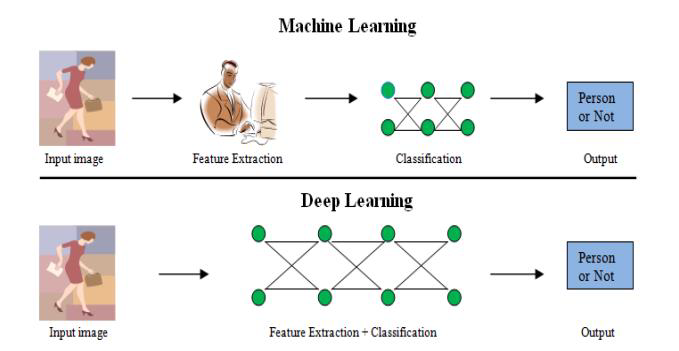
\includegraphics[width=0.8\textwidth]{img/2-Antecedentes/2.1-Estado_arte/ML_vs_DL.png}
    \caption{Machine Learning vs Deep Learning \cite{gupta2022deep}}
    \label{fig:2.1-ML_vs_DL}
\end{figure}

\par La detección de fallas en correas transportadoras se aborda como un problema de detección de objetos mediante aprendizaje supervisado. Existen dos enfoques principales: los modelos de dos etapas, como la familia R-CNN (red neuronal convolucional basada en regiones), que emplean redes de propuestas regionales seguidas de refinamiento, y los modelos de una etapa, como YOLO y SSD, que realizan predicciones por regresión directa, optimizados para aplicaciones en tiempo real \cite{zhang2021deep}. \\

\par La detección de objetos ha sido uno de los problemas centrales en visión por computadora, tradicionalmente abordado mediante arquitecturas basadas en redes neuronales convolucionales (CNN). Estos modelos dominaron el campo durante más de una década, impulsando desarrollos significativos en precisión y eficiencia. Sin embargo, alcanzar un balance óptimo entre velocidad y exactitud ha requerido explorar estructuras más allá del marco convencional de las CNN. Los modelos basados en transformers, originalmente desarrollados para procesamiento de lenguaje natural (Natural Language Processing), han demostrado ser altamente efectivos al capturar relaciones espaciales globales en imágenes, lo que los convierte en una propuesta a considerar para la implementación de nuevos modelos de detección de objetos \cite{arkin2023survey}. \\

\par Una memoria de título desarrollada en la Universidad de Chile \cite{angulo2024deteccion} implementa visión computacional y técnicas de aprendizaje profundo (Deep Learning) para la detección temprana de fallas en correas transportadoras, utilizando una de las versiones del modelo YOLO (You Only Look Once). El estudio describe detalladamente la implementación y calibración del modelo, además de proporcionar información técnica sobre redes neuronales convolucionales, métricas de evaluación, pruebas experimentales y resultados ilustrativos.

%%%%%%%%%%%%%%%%%%%%%%%%%%%%%%%%%%%%%%%%%%%%%%%
\subsection{Fallas en correas transportadoras}

\par Las correas transportadoras operan en condiciones que las exponen a diversos tipos de daños, los cuales pueden generar costosos tiempos de inactividad. Para cada condición de falla, se han revisado exhaustivamente sus tipos y causas, así como los métodos adecuados para su mitigación, contribuyendo a mejorar la confiabilidad del sistema \cite{khanna2022types}. \\

\par Entre las fallas más comunes en correas transportadoras se identifican el \textbf{daño por impacto}, que puede provocar \textbf{perforaciones o roturas locales}; la \textbf{delaminación}, generada por esfuerzos cíclicos y fatiga; y la \textbf{desalineación de la banda}, que causa \textbf{desgaste anómalo en los bordes}. Además, se reporta \textbf{desgaste abrasivo} en la cubierta superior por efecto de partículas duras, \textbf{rotura de cables de acero} en correas reforzadas, y \textbf{cortes longitudinales y transversales}, todos los cuales afectan directamente la vida útil y seguridad operativa del sistema.


\begin{figure}[H]
    \centering
    \subfloat[Desgasta abrasivo banda]{
        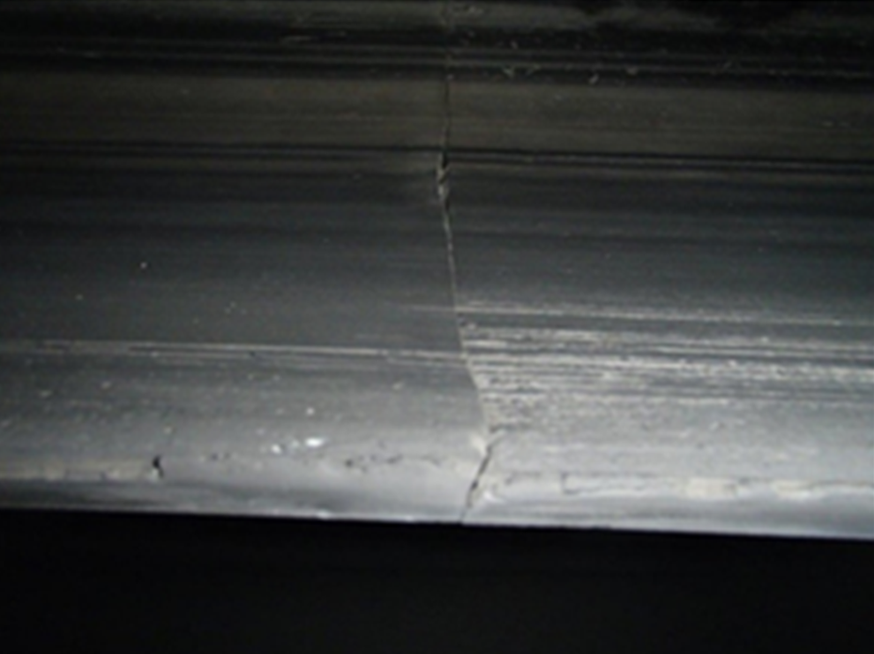
\includegraphics[width=0.23\textwidth]{img/2-Antecedentes/Fotos_Fallas/Desgaste_abrasivo_banda.png}
    }
    \hfill
    \subfloat[Desgaste abrasivo bordes banda]{
        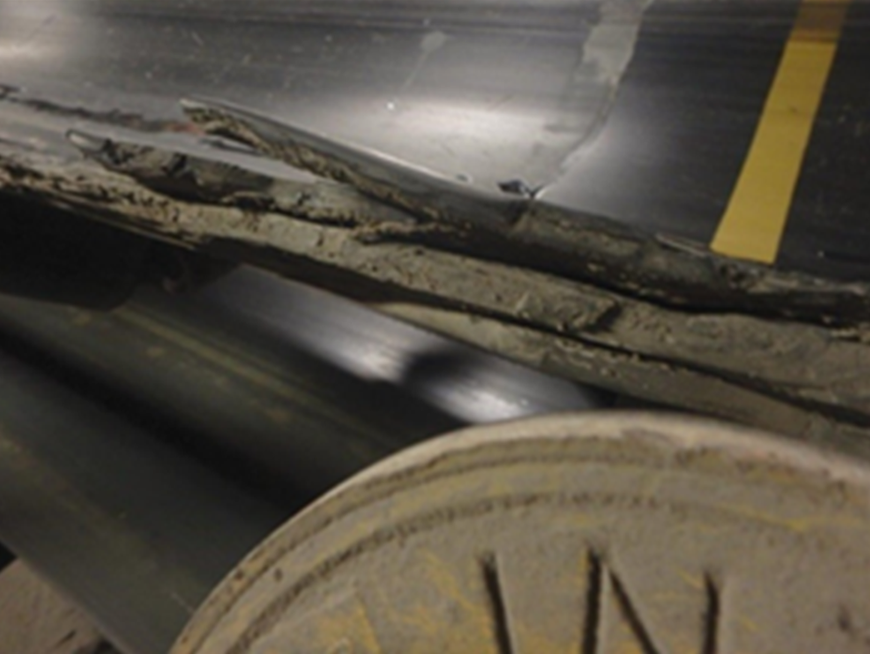
\includegraphics[width=0.23\textwidth]{img/2-Antecedentes/Fotos_Fallas/Desgaste_abrasivo_banda_bordes.png}
    }
    \hfill
    \subfloat[Perforación de banda]{
        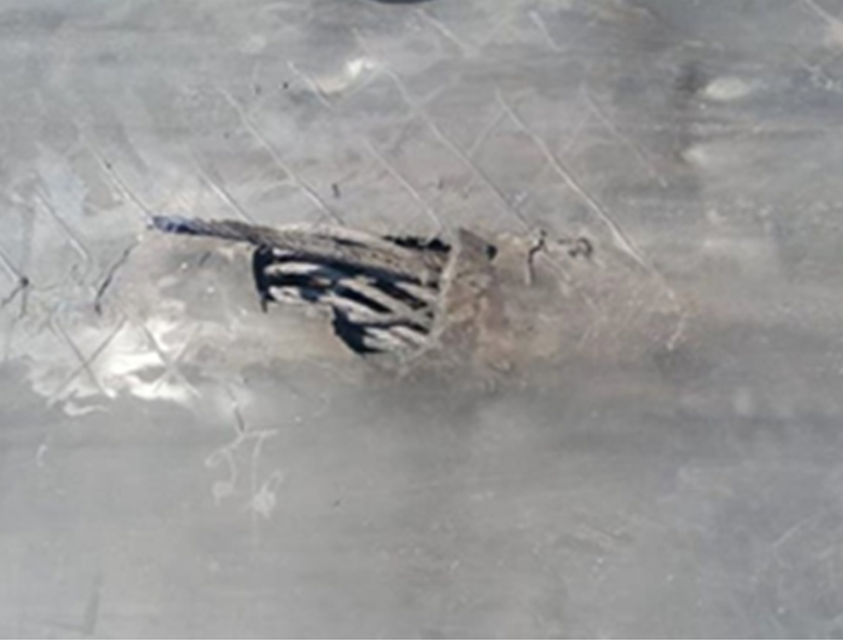
\includegraphics[width=0.23\textwidth]{img/2-Antecedentes/Fotos_Fallas/Perforacion_banda.png}
    }
    \hfill
    \subfloat[Rotura de banda]{
        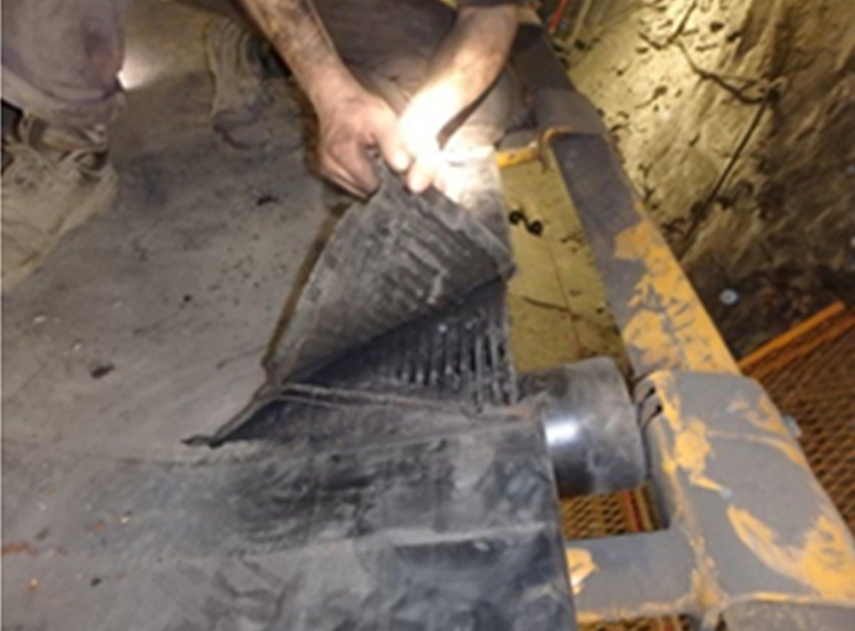
\includegraphics[width=0.23\textwidth]{img/2-Antecedentes/Fotos_Fallas/Rotura_banda.png}
    }
    \hfill
    \subfloat[Corte longitudinal ó Desgarro]{
        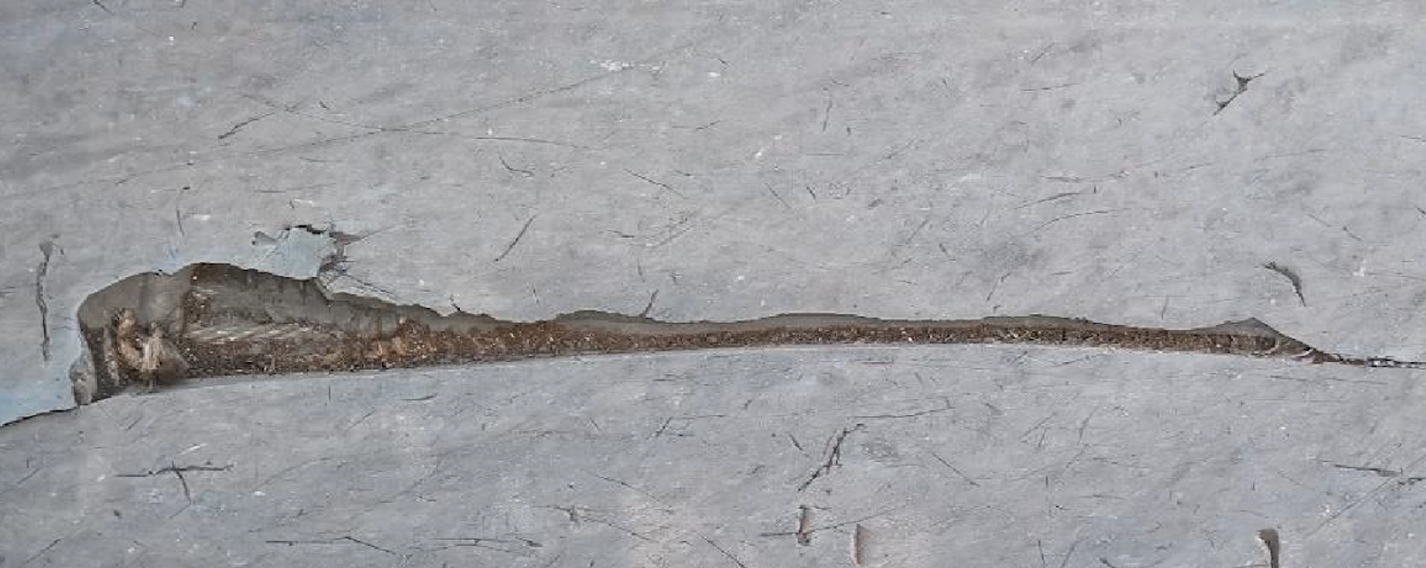
\includegraphics[width=0.4\textwidth]{img/2-Antecedentes/Fotos_Fallas/Corte_longitudinal.png}
    }
    \caption{Tipos de falla comunes en correas transportadoras, imágenes adaptadas de \cite{khanna2022types}.}
    \label{fig:falla_correas}
\end{figure}
%%%%%%%%%%%%%%%%%%%%%%%%%%%%%%%%%%%%%%%%%%%%%%%%%

\section{Redes Neuronales Convolucionales (CNN)}

\subsection{Arquitectura}

\par La detección de objetos en visión por computadora consiste en identificar automáticamente instancias u objetos presentes en una imagen o secuencia, localizándolos mediante cajas delimitadoras y asignándoles una clase. En los modelos modernos, esta tarea se formula como un problema conjunto de clasificación y regresión: para cada región candidata de la imagen se predice la probabilidad de pertenencia a una clase y las coordenadas de la caja delimitadora asociada. Para abordar este problema de manera eficiente, las arquitecturas actuales separan conceptualmente el modelo en dos bloques: (i) un \textit{backbone} convolucional que extrae mapas de características jerárquicos desde la imagen de entrada y (ii) una o varias cabezas de detección encargadas de proyectar dichos mapas en predicciones de clases y cajas delimitadoras \cite{kaur2022tools,lubinus2023redes}. \\

\begin{figure}[H]
    \centering
    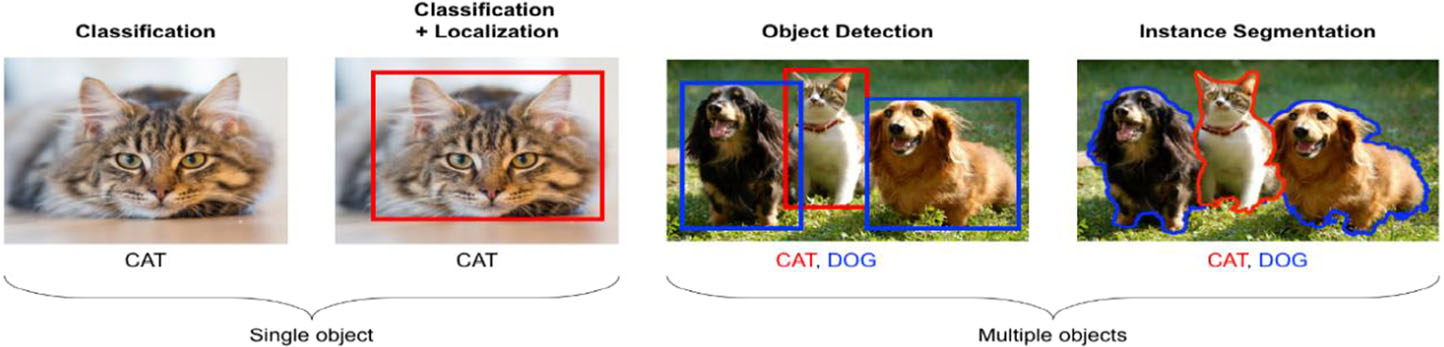
\includegraphics[width=0.9\textwidth]{img/2-Antecedentes/2-Object_Detection_example.png}
    \caption{Ejemplos de detección de objetos simples y múltiples. Imagen adaptada de \cite{kaur2022tools}.}
    \label{fig:2.2-object_detection_example}
\end{figure}

\par En este contexto, las redes neuronales convolucionales (CNN) constituyen el núcleo de la mayoría de arquitecturas de visión por computador. Una CNN está formada por una sucesión de capas de convolución, funciones de activación no lineales (como ReLU o variantes), capas de normalización y, en algunos casos, capas de reducción de dimensionalidad (\textit{pooling}). Las convoluciones aplican filtros o \textit{kernels} que se desplazan sobre la imagen, compartiendo pesos en el plano espacial. Este mecanismo reduce el número de parámetros, explota la estructura local de las imágenes y confiere invariancia aproximada a traslaciones \cite{lubinus2023redes}. \\

\par Tal como se describe en revisiones recientes de aprendizaje profundo, las primeras capas de una CNN tienden a aprender características de bajo nivel (bordes, texturas, gradientes de intensidad), mientras que las capas intermedias y profundas capturan patrones de mayor complejidad (formas, partes de objetos y, finalmente, representaciones semánticas de alto nivel). Este aprendizaje jerárquico permite que una misma arquitectura pueda generalizar sobre grandes volúmenes de datos y adaptarse a distintas tareas visuales mediante el ajuste de sus parámetros \cite{gupta2022deep,lubinus2023redes}. \\

\par En las capas de reducción o \textit{pooling}, como el \textit{max pooling}, se disminuye la resolución espacial de los mapas de características conservando las activaciones más relevantes. Esta etapa reduce la carga computacional y actúa como un mecanismo de regularización, al atenuar pequeños desplazamientos o deformaciones locales en la imagen. Finalmente, uno o varios bloques de capas densas (\textit{fully connected}) agregan la información extraída y realizan la clasificación o regresión final, según el diseño del modelo \cite{lubinus2023redes}. \\

\par Para tareas de detección de objetos, las CNN se integran habitualmente en una arquitectura de tipo \textit{backbone--neck--head}. El \textit{backbone} (por ejemplo, variantes de VGG, ResNet u otras arquitecturas optimizadas para eficiencia) extrae los mapas de características base. Sobre estos mapas, el \textit{neck} construye representaciones multiescala mediante estructuras como pirámides de características (FPN, PAN), lo que permite detectar objetos de distintos tamaños. Finalmente, la \textit{head} de detección proyecta esas características a predicciones de clases y cajas delimitadoras, como ocurre en los modelos de una sola etapa (\textit{single-shot}) tipo YOLO y SSD, descritos en secciones posteriores \cite{zhang2021deep}. \\

\subsection{Hiperparámetros comunes}

\par Las arquitecturas basadas en CNN dependen de un conjunto de hiperparámetros que controlan tanto la forma de la red como el proceso de entrenamiento. A diferencia de los parámetros internos del modelo (pesos y sesgos), los hiperparámetros se fijan externamente y condicionan la calidad de las representaciones aprendidas, la velocidad de convergencia y el grado de generalización. En aplicaciones de detección de objetos, la adecuada configuración de estos hiperparámetros resulta crítica para lograr un equilibrio entre precisión y costo computacional \cite{gupta2022deep,zhang2021deep}. \\

\par En la práctica, muchos de estos hiperparámetros son compartidos por distintas arquitecturas de detección basadas en CNN (por ejemplo, SSD, YOLO o variantes híbridas), lo que permite definir configuraciones iniciales razonables y posteriormente ajustarlas de forma iterativa. La Tabla \ref{tab:2-hiperparametros-comunes-cnn} resume algunos de los hiperparámetros más habituales, junto con rangos típicos y una descripción de su efecto sobre el entrenamiento del modelo. \\

\begin{table}[H]
    \centering
    \caption{Hiperparámetros comunes en modelos de detección basados en CNN}
    \begin{tabular}{|c|c|c|}
        \hline
        \textbf{Hiperparámetro} & \textbf{Rango típico} & \textbf{Nombre} \\ 
        \hline
        $lr0$ & $10^{-5}$ -- $10^{-1}$ & Tasa de aprendizaje inicial \\ 
        \hline
        $lrf$ & 0,01 -- 1,0 & Factor de tasa final \\ 
        \hline
        Número de \textit{épocas} & 100 -- 150 & \textit{Épocas} de entrenamiento \\ 
        \hline
        Tamaño de imagen & $640 \times 640$ píxeles & Resolución de entrada \\ 
        \hline
        Tamaño de \textit{batch} & 4 / 8 / 16 imágenes & Tamaño de lote (\textit{batch}) \\ 
        \hline
        $weight\_decay$ & 0,0 -- 0,001 & Regularización $L_2$ \\ 
        \hline
        $box\_loss$ & 0,02 -- 0,2 & Peso pérdida de cajas \\ 
        \hline
        $cls\_loss$ & 0,02 -- 4,0 & Peso pérdida de clasificación \\ 
        \hline
        $object\_loss$ & 0,02 -- 0,04 & Peso pérdida de objeto \\ 
        \hline
        $warmup\_epochs$ & 0 -- 5 & \textit{Épocas} de calentamiento \\ 
        \hline
    \end{tabular}
    \label{tab:2-hiperparametros-comunes-cnn}
\end{table}





%%%%%%%%%%%%%%%%%%%%%%%%%%%%%%%%%%%%%%%%%%%%%%%
\section{Mecanismo de atención y arquitectura Encoder-Decoder}

\subsection{Mecanismo de atención en transformers}

\par Los modelos modernos basados en transformers utilizan mecanismos de auto-atención para ponderar de manera dinámica la relevancia de cada elemento de la entrada con respecto a los demás. En el contexto de visión por computador, la imagen se representa como una secuencia de \textit{tokens} (por ejemplo, parches proyectados a un espacio de embeddings), sobre los cuales la auto-atención estima qué regiones resultan más informativas para la tarea. Este esquema permite capturar dependencias espaciales de largo alcance, superando la limitación local de los filtros convolucionales clásicos. \\

\par Debido a la complejidad de estos mecanismos, han surgido métodos de explicabilidad que permiten visualizar la contribución de cada token de entrada en la inferencia. Entre ellos, se propone un enfoque general aplicable a arquitecturas bi-modales y encoder-decoder, capaz de generar mapas de atención interpretables a partir de las ponderaciones internas del modelo. Estas herramientas de interpretabilidad resultan especialmente útiles en arquitecturas de detección basadas en transformers, donde la distribución de la atención sobre la imagen entrega información complementaria sobre las regiones que influyen en la predicción final \cite{chefer2021generic}. \\

\subsection{Arquitecturas encoder-decoder para detección de objetos}

\par En tareas de detección de objetos, los transformers suelen organizarse bajo un esquema encoder-decoder. Modelos como DETR y DINO utilizan un codificador (\textit{encoder}) que transforma la imagen en una representación latente mediante auto-atención, y un decodificador (\textit{decoder}) que cruza estas representaciones con un conjunto fijo de consultas (\textit{object queries}) para predecir directamente las clases y localizaciones de los objetos presentes. De este modo, el problema de detección se formula como un mapeo directo entre un conjunto de consultas y las instancias de objetos en la imagen, evitando componentes manuales como los algoritmos de propuestas de regiones \cite{carion2020end,zhang2022dino}. \\

\par En versiones más recientes, como DINO, se introducen mejoras sobre el esquema original de DETR mediante el uso de extractores de características multiescala, atención deformable y estrategias de entrenamiento con ramas de desruido (\textit{denoising}). Estas extensiones permiten una convergencia más rápida y una gestión más robusta de muestras difíciles, manteniendo la formulación encoder-decoder como eje central de la arquitectura \cite{zhang2022dino}. \\

\par De manera complementaria, la destilación de conocimiento (\textit{knowledge distillation}) se ha incorporado como una estrategia para transferir la capacidad representacional de modelos visuales de gran escala (\textit{teacher}) hacia arquitecturas más livianas y eficientes (\textit{student}). En el contexto de la detección de objetos con transformers, esta técnica permite condensar el conocimiento aprendido por modelos preentrenados en clasificación o detección sobre grandes bases de datos, reduciendo el costo computacional en la inferencia sin sacrificar significativamente el rendimiento \cite{li2024distilling}. \\




%%%%%%%%%%%%%%%%%%%%%%%%%%%%%%%%%%%%%%%%%%%%%%%
\clearpage
\section{Modelos de detección de objetos de una sola etapa (YOLO y SSD)}


\subsection{Contextualización}


\par YOLO y SSD pertenecen a la familia de modelos de detección de objetos de una sola etapa (\textit{one-stage detectors}), en los cuales la localización de las cajas delimitadoras y la clasificación de las instancias se realizan en una única pasada por la red. Ambos se basan en redes neuronales convolucionales (CNN) y se enmarcan dentro de los enfoques de detección de objetos con aprendizaje profundo (\textit{Deep Learning}), donde la propia red efectúa de manera conjunta la extracción de características y la predicción final. En la Figura~\ref{fig:2.4-YOLO_SSD_DL} se esquematiza la relación entre los esquemas tradicionales de detección de objetos basados en \textit{Machine Learning}, los modelos de una etapa como YOLO y SSD —que serán objeto de estudio en esta memoria— y los modelos de dos etapas (\textit{two-stage}), dentro de los cuales destaca la familia R-CNN, pionera en el uso de propuestas de regiones como base para la extracción de características y la detección posterior \cite{kaur2022tools}. \\

\begin{figure}[H]
    \centering
    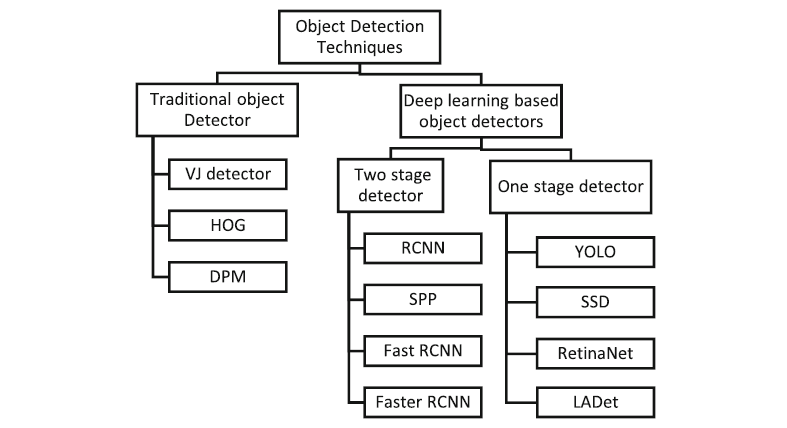
\includegraphics[width=0.8\textwidth]{img/2-Antecedentes/2.4-YOLO_SSD/YOLO_SSD_DL.png}
    \caption{Clasificación de varias técnicas de detección de objetos. Imagen extraída de \cite{kaur2022tools}.}
    \label{fig:2.4-YOLO_SSD_DL}
\end{figure}



\subsection{YOLO (You Only Look Once)}

\par YOLO (You Only Look Once) es un enfoque de detección de objetos de una sola etapa que destaca por su alta velocidad y eficiencia, al predecir directamente las clases y ubicaciones de objetos en una sola pasada por la red. A diferencia de métodos de dos etapas como R-CNN o Faster R-CNN, YOLO evita la generación de propuestas de regiones, lo que lo hace apto para aplicaciones en tiempo real. Su arquitectura unificada lo convierte en una opción balanceada entre precisión y velocidad \cite{terven2023comprehensive}.\\

\par 

\begin{figure}[H]
    \centering
    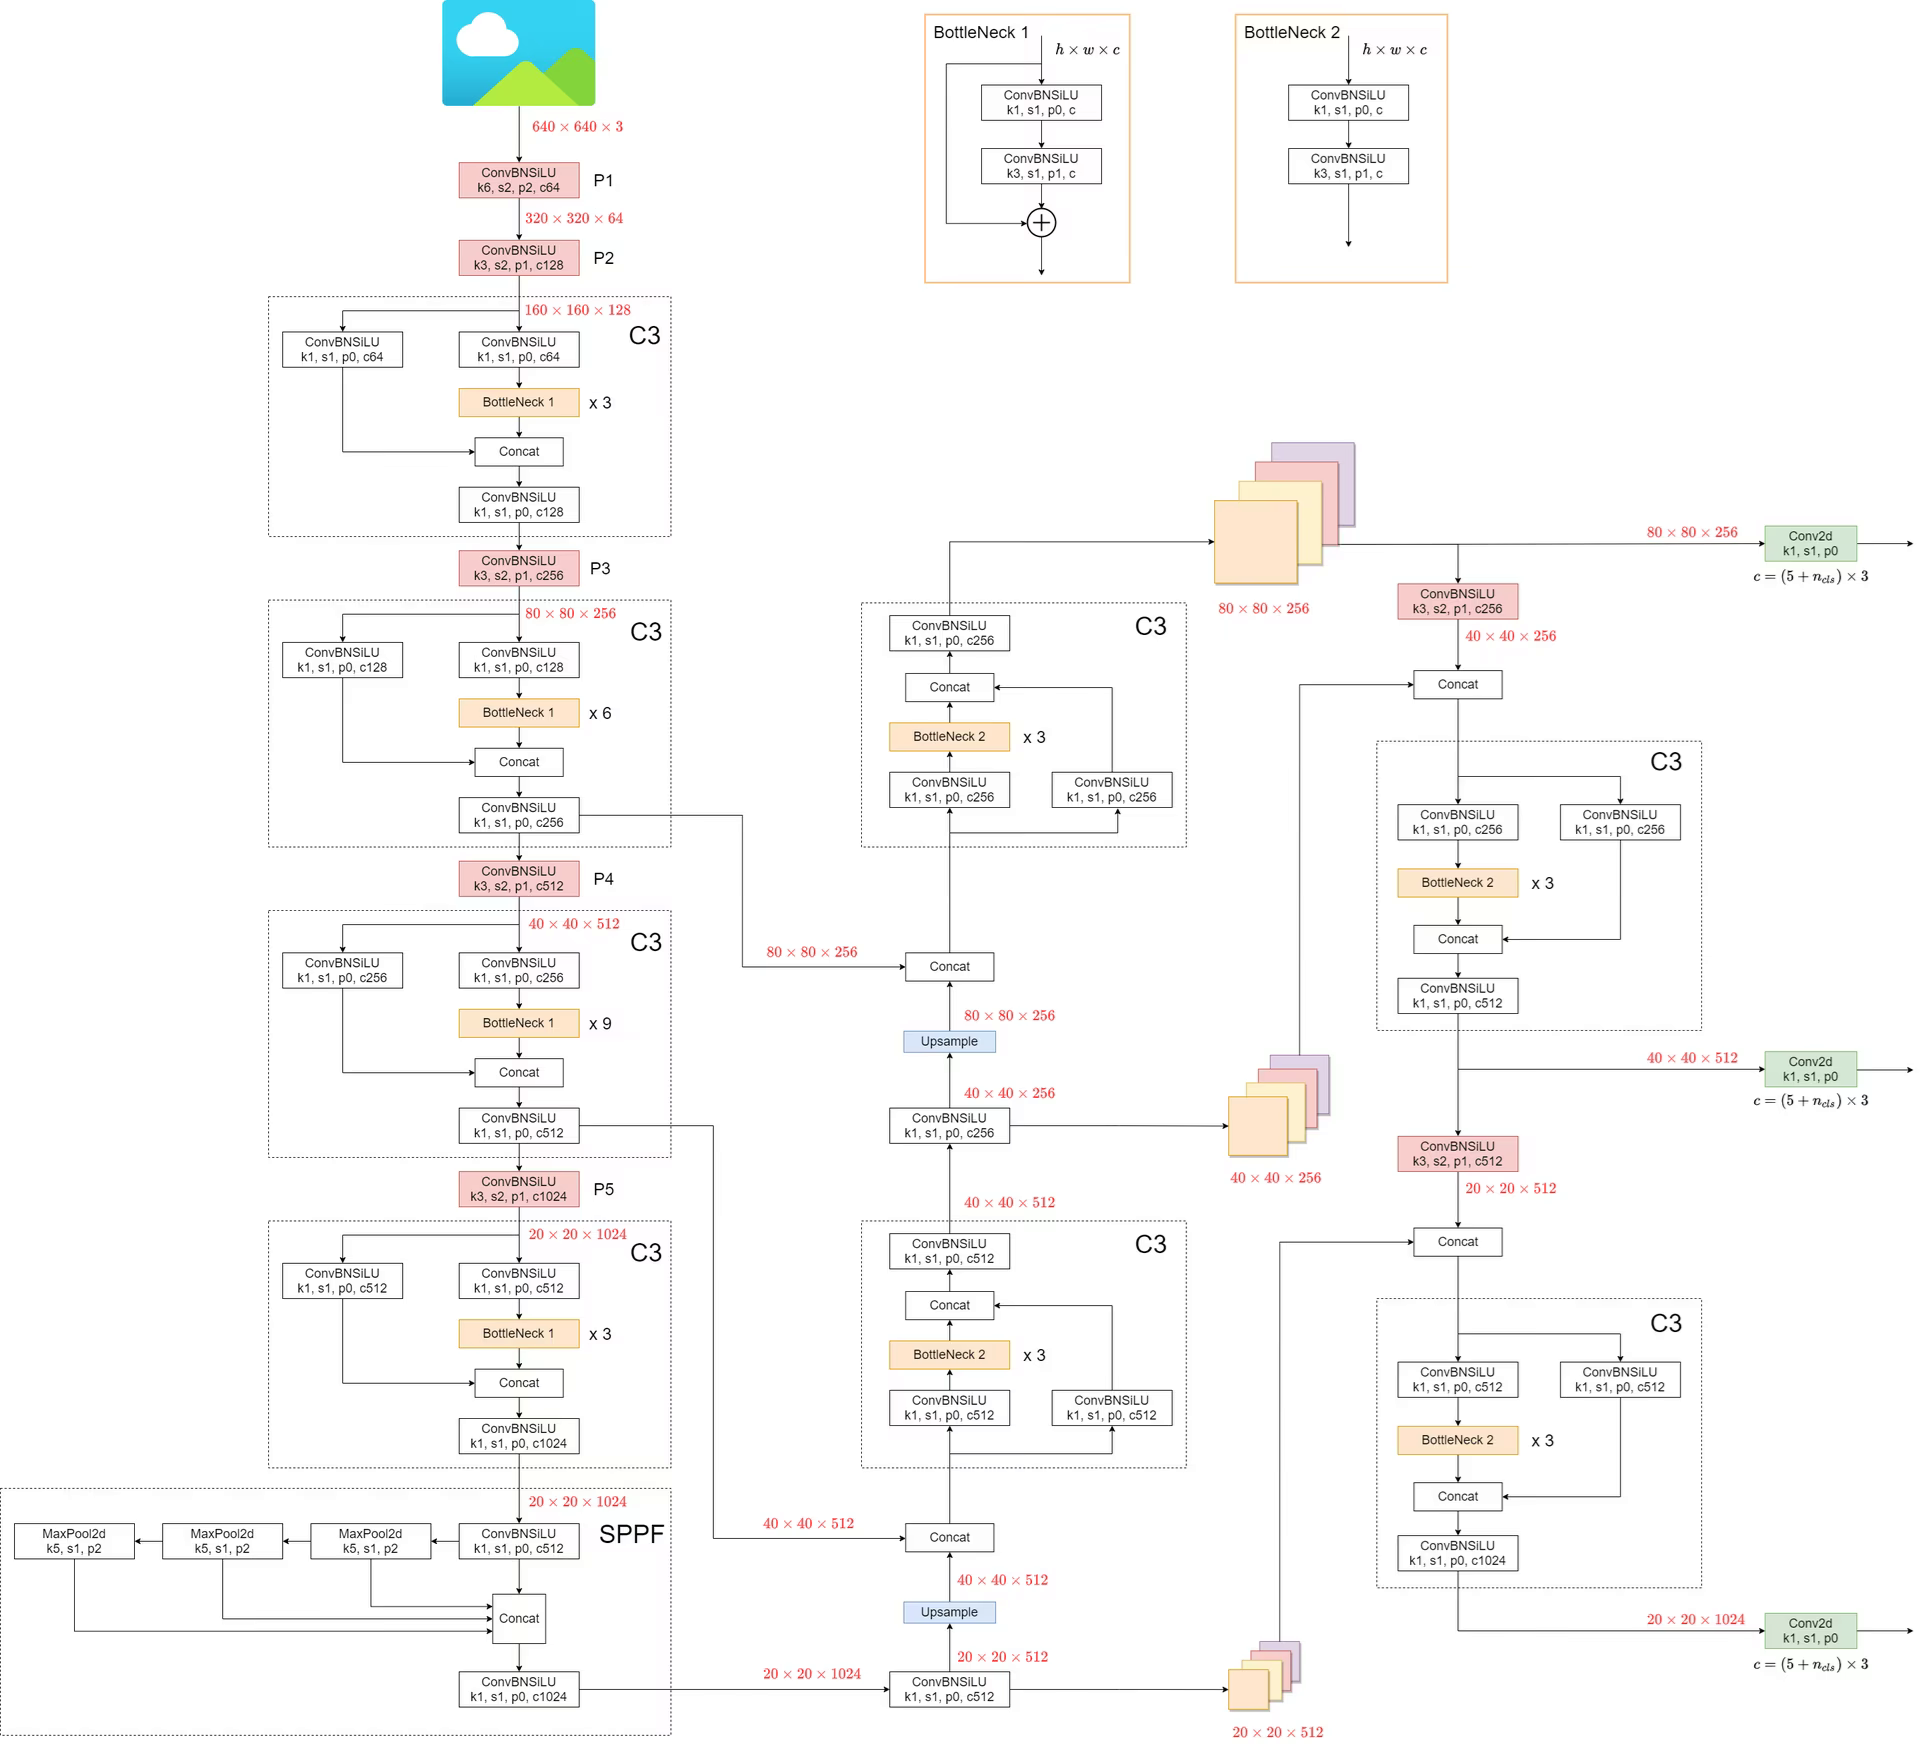
\includegraphics[width=0.9\textwidth]{img/2-Antecedentes/2.4-YOLO_SSD/YOLO_v5_Architecture_l.png}
    \caption{Arquitectura de YOLOv5.}
    \label{fig:2.4-YOLO_v5_architecture}
\end{figure}



\subsection{SSD (Single Shot Multibox Detector)}

\par SSD (Single Shot Multibox Detector) es otro enfoque en la detección de objetos, caracterizado por su capacidad de realizar clasificación y regresión de cajas delimitadoras en una única pasada de la red, sin requerir etapas de propuesta de regiones. SSD utiliza múltiples mapas de características de diferentes escalas para detectar objetos de diversos tamaños, lo que mejora la precisión especialmente en objetos pequeños \cite{liu2016ssd}. La arquitectura general (que contempla sus dos versiones), se muestra en la Figura \ref{fig:2.4-SSD_architecture}.
  
\begin{figure}[H]
    \centering
    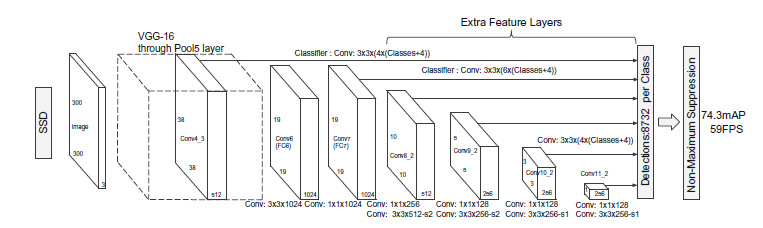
\includegraphics[width=0.8\textwidth]{img/2-Antecedentes/2.4-YOLO_SSD/SSD_Architecture.png}
    \caption{Arquitectura general de SSD. Imagen extraída y procesada de \cite{liu2016ssd}.}
    \label{fig:2.4-SSD_architecture}
\end{figure}

\par 

\subsection{Hiperparámetros}

\par Los hiperparámetros son valores que controlan el proceso de aprendizaje y condicionan los parámetros internos que el modelo ajusta durante el entrenamiento. Se denominan así por encontrarse en un nivel superior, ya que no forman parte del modelo aprendido, sino que guían su optimización. Al finalizar el entrenamiento, el modelo resultante contiene únicamente los parámetros ajustados, mientras que los hiperparámetros utilizados permanecen externos a dicha estructura \cite{nyuytiymbiy2020parameters}.
\\

\par El ajuste de hiperparámetros en los modelos de detección de objetos basados en redes neuronales convolucionales, es un proceso iterativo el cual está destinado a optimizar las métricas de evaluación utilizadas en visión computacional \cite{ultralytics2025hyperparam}.


%%%%%%%%%%%%%%%%%%%%%%%%%%%%%%%%%%%%%%%%%%%%%%%
\section{DETR (DEtection TRansformer) y DINO}

\subsection{Arquitecturas}

\par DETR y DINO son modelos de detección de objetos basados en la arquitectura de transformers, originalmente desarrollada para procesamiento de lenguaje natural, pero adaptada para visión por computadora. 
\\

%DETR
\par DETR (DEtection TRansformer) es un modelo de aprendizaje profundo (deep-learning), compuesta por tres elementos principales: un backbone convolucional (CNN backbone) que extrae las representaciones visuales, un transformador encoder-decoder (encoder-decoder transformer) que modela relaciones globales en la imagen, y una red neuronal completamente conectada (feed forward network, FFN) que realiza las predicciones finales. DETR no requiere componentes manuales ni estructuras complejas, lo que permite su implementación en frameworks de aprendizaje profundo estándar con pocas líneas de código \cite{carion2020end}. \\

%DINO

\par DINO es un modelo basado en DETR que incluye un backbone, un encoder y decoder multi-capa de Transformer, y múltiples cabezas de predicción (prediction heads). Emplea extractores de características multiescala que se procesan con embeddings posicionales (positional embeddings) en el encoder. Su innovación principal. respecto a DETR, es la selección mixta de queries (solicitudes) para inicializar anclas posicionales (positional anchors) en el decoder, mientras que las queries de contenido (content queries) permanecen aprendibles. Utiliza atención deformable (deformable attention) para actualizar características capa a capa y cuenta con una rama de desruido (denoising) con entrenamiento contrastivo, mejorando la gestión de muestras difíciles \cite{zhang2022dino}.



\subsection{Hiperparámetros}

\par En el modelo DETR, los hiperparámetros incluyen configuraciones específicas del número de \textit{layers} (capas) en la arquitectura, tasas de \textit{regularization} (regularización), tipo de \textit{optimizer} (optimizador) y esquemas de \textit{data augmentation} (aumento de datos) \cite{carion2020end}.
\\

\par En el modelo DINO, los hiperparámetros comparten similitudes con DETR, incluyendo el uso del optimizador AdamW con regularización por decaimiento de peso (weight decay) y ajustes en la tasa de aprendizaje mediante un programador dinámico (learning rate scheduler). Además, DINO incorpora un conjunto fijo y ampliado de consultas para el decoder (decoder queries), optimizando el equilibrio entre desempeño y costo computacional durante el entrenamiento \cite{zhang2022dino}.
%%%%%%%%%%%%%%%%%%%%%%%%%%%%%%%%%%%%%%%%%%%%%%
\section{Métricas}

\par Con el fin de validar la implementación de los modelos de detección de objetos para la clasificación de fallas, se emplean métricas cuantitativas estándar en visión por computador. El uso de estas métricas otorgan las herramientas esenciales para evaluar críticamente y de forma fiable los modelos implementados \cite{schlosser2024overview}.

\subsection{Precisión, Exhaustividad y F-Score}

\par La \textbf{precisión} (\textit{precision}) mide la proporción de verdaderos positivos entre todas las predicciones positivas. El \textbf{recall} o \textit{exhaustividad} mide la proporción de verdaderos positivos detectados sobre los positivos reales. 

\[
\text{Precision} = \frac{TP}{TP + FP} \quad \quad \text{Recall} = \frac{TP}{TP + FN}
\]

\begin{table}[H]
    \centering
    \begin{tabular}{|c|c|}
        \hline
         \textbf{Abreviación} & \textbf{Significado}  \\
         \hline
         T & Total \\
         \hline
         P & Positivos \\
         \hline
         N & Negativos \\
         \hline
         TP & Verdaderos Positivos \\
         \hline
         TN & Verdaderos Negativos \\
         \hline
         FP & Falsos Negativos \\
         \hline
         n & Número de Clases \\
         \hline
    \end{tabular}
    \caption{Definiciones generales \textit{Machine Learning} \cite{schlosser2024overview}}
    \label{tab:2-def_metricas}
\end{table}


\par El \textbf{F-Score} ($F_{\beta}$) es la media ponderada entre precisión y recall, ajustada por el parámetro $\beta$. Un caso particular es el \textbf{F1-Score} ($F_{1}$), donde $\beta = 1$.

\[
F_{\beta} = (1 + \beta^2) \cdot \frac{\text{Precision} \cdot \text{Recall}}{\beta^2 \cdot \text{Precision} + \text{Recall}} \quad \quad F_1 = 2 \cdot \frac{\text{Precision} \cdot \text{Recall}}{\text{Precision} + \text{Recall}}
\]

\subsection{IoU y Confianza}

\par El \textbf{IoU (Intersection over Union)} evalúa el solapamiento entre la predicción y la verdad de terreno:
\\
\[
\text{IoU} = \frac{\text{Área de Intersección}}{\text{Área de Unión}}
\]

\par La \textbf{confianza} asigna una probabilidad a la predicción, y el \textbf{umbral de confianza} define el valor mínimo para aceptar una detección.

\subsection{AP y mAP}

\par La \textbf{Average Precision (AP)} corresponde al área bajo la curva precisión-recall para una clase. El \textbf{mean Average Precision (mAP)} es el promedio del AP para todas las clases. \\

\par El \textbf{mAP@50} utiliza un umbral IoU fijo de 0{,}5. \textbf{mAP@50-95} promedia el AP en umbrales de IoU entre 0{,}5 y 0{,}95 (paso de 0{,}05), reflejando un criterio más exigente y robusto.

\subsection{Matriz de Confusión}

\par Representa los aciertos y errores del clasificador mediante los conteos de verdaderos/falsos positivos y negativos por clase, permitiendo un análisis detallado del comportamiento del modelo.

\chapter{Metodología}

%%%%%%%%%%%%%%%%%%%%%%%%%%%%%%%%%%%%%%%%%
\section{Identificación de fallas}

\par De acuerdo al Capítulo 2, sección 2.1, las fallas en correas transportadoras se encuentran enmarcadas de acuerdo a \cite{khanna2022types} y para la implementación de modelos de reconocimiento de objetos que identifiquen estaas fallas, se consideraron las siguientes fallas:

\begin{itemize}
    \item Agujero (Hole): pérdida completa de material a través del espesor de la banda, de tamaño apreciable, originada por eventos de daño severo (impactos altos, atrapamiento de material o elementos extraños).
    \item Daño por impacto (Impact Damage): deformaciones, cortes o abrasiones localizadas en la zona de carga, producidas por el impacto repetitivo o puntual del material transportado.
    \item Perforación (Puncture): daño puntual en el que un elemento punzante atraviesa la banda generando una abertura de menor extensión superficial que un agujero, usualmente de carácter incipiente.
    \item Desgarro (Tear): separación longitudinal o transversal de la banda, asociada a sobrecargas, material atascado o concentraciones de tensión, y que puede propagarse a lo largo de la correa.
    \item Abrasión (Wear): desgaste progresivo de la superficie de la correa debido a fricción, que se manifiesta como adelgazamiento del recubrimiento y patrones característicos de pérdida de material.
\end{itemize}

\par De esta forma, las fallas antes mencionadas se convierten en \textit{clases} para los modelos de detección de objetos.

%%%%%%%%%%%%%%%%%%%%%%%%%%%%%%%%%%%%%%%%%
\section{Base de datos y entorno virtual}


\subsection{Base de datos elaborada}
\par El entrenamiento de modelos basados en redes neuronales (convolucionales o no) requiere disponer de un conjunto de datos suficientemente representativo, anotado y particionado en subconjuntos mutuamente excluyentes:

\begin{itemize}
    \item \textbf{Entrenamiento (train)}: conjunto utilizado para ajustar los parámetros del modelo mediante el proceso de optimización. Suele concentrar entre un 60\% y un 80\% del total de muestras disponibles.
    \item \textbf{Validación (valid)}: conjunto empleado durante el entrenamiento para calcular métricas intermedias, seleccionar hiperparámetros y monitorizar el sobreajuste. Sus ejemplos no se usan para actualizar los pesos del modelo y, por lo general, representan una fracción menor que el conjunto de entrenamiento.
    \item \textbf{Prueba (test)}: conjunto reservado para la evaluación final e independiente del modelo, una vez completado el ajuste y la selección de hiperparámetros. Permite estimar el desempeño esperado en condiciones de uso real.
\end{itemize}


\subsection{Recopilación y limpieza}

\par Mediante el sitio web \textit{Roboflow}, así como plataformas de datos abiertos tales como \textit{Kaggle Datasets}, \textit{ImageNet}, \textit{Open Images Dataset} y otros repositorios académicos de libre acceso, se recopilaron bases de datos relacionadas con fallas en correas transportadoras y con entornos industriales de transporte de material a granel. Cada conjunto presentaba su propia organización de clases, resolución de imágenes y formato de anotación, por lo que fue necesario unificar las etiquetas al formato YOLO antes de su utilización en los modelos de detección. \\

\par Posteriormente, se aplicó un proceso de depuración y limpieza de datos. En primer lugar, se descartaron imágenes irrelevantes (sin presencia clara de correa transportadora o sin defecto observable) y aquellas con problemas severos de calidad, como baja resolución, desenfoque o ruido excesivo. En segundo lugar, se normalizaron las anotaciones corrigiendo etiquetas inconsistentes, reclasificando ejemplos cuya clase no coincidía con el defecto presente y ajustando las cajas delimitadoras cuando su posición o tamaño eran inadecuados. Finalmente, se homogeneizó la nomenclatura de clases y el formato de las etiquetas, garantizando una base de datos coherente y consistente para el entrenamiento y evaluación de los modelos. \\

\par En total, se logró confeccionar una base de datos de 2312 imágenes, todas con resolución de 640x640px y etiquetas normalizadas de acuerdo al formato que usa YOLO.


%%%%%%%%%%%%%%%%%%%%%%%%%%%%%%%%%%%%%%%%%%%%%%%%%%%%%

\subsection{Entorno virtual}

\par Con el fin de asegurar la reproducibilidad de los experimentos y aislar las dependencias del proyecto, se implementó un entorno virtual basado en \textit{Python} en la raíz del repositorio \textit{Implementation-of-Object-Recognition-Algorithms-for-Conveyor-Belt-Defect-Detection}. Todas las librerías requeridas se gestionan mediante el archivo de requerimientos (\textit{Environment/requirements.txt}), que agrupa paquetes para aprendizaje profundo, procesamiento de datos, visión por computador y visualización de resultados. \\

\par La creación y activación del entorno se realiza con las utilidades estándar de \textit{Python} y la instalación automatizada de dependencias a partir de \textbf{Environment/requirements.txt}. La ejecución de los modelos se efectúa sobre una GPU AMD Radeon compatible con la pila ROCm/DirectML, utilizando la distribución oficial de PyTorch para esta plataforma.




%%%%%%%%%%%%%%%%%%%%%%%%%%%%%%%%%%%%%%%%%%%%%%%
\section{Implementación de YOLOv5}

\subsection{Estructura de trabajo}

\par La implementación de YOLOv5 desde el modelo oficial de Ultralytics en el ambiente actual sigue la estructura de trabajo mostrada en el Código \ref{lst:estructura-yolov5}. El modelo oficial de YOLOv5 se guarda en una carpeta dentro de YOLO. Posteriormente, se configuran todos los archivos necesarios a modo de capa envolvente del modelo original para poder utilizarlo de manera compatible al entorno virtual. \\


\begin{lstlisting}[
    float,
    floatplacement=H,                               
    caption={Estructura de directorios para la implementación de YOLO.},
    label={lst:estructura-yolov5},
    basicstyle=\ttfamily\scriptsize,
    numbers=none,                            % sin numeracion de lineas
    columns=fullflexible,
    frame=single,
    xleftmargin=2.5cm,
    framexleftmargin=0.5cm,
    framexrightmargin=0.5cm,
    breaklines=true,
    breakatwhitespace=true
]
YOLO/
|-- configs/
|   |-- dataset.yaml        : Rutas y clases del dataset
|   |-- model_variants.yaml : Parametros de escalado (variantes)
|   |-- train.yaml          : Hiperparametros de entrenamiento
|   `-- valid.yaml          : Hiperparametros de validacion
|-- engine/
|   |-- bn2gn_patch.py      : Parche para normalizacion por lotes
|   |-- bootstrap_miopen.py : Interfaz de mitigacion de MIOpen
|   |-- Trainer.py          : Modulo de entrenamiento
|   |-- Validator.py        : Modulo de validacion interna/externa
|   `-- warnings.py         : Modulo de advertencias y errores menores
|-- metrics/                : Carpeta de almacenamiento de metricas
|-- runs/                   : Carpeta de almacenamiento de ejecuciones
|-- utility/
|   |-- check_dataset.py    : Revisa formato dataset para modelo a entrenar
|   |-- clean_logs_runs.py  : Script de limpieza de logs y runs
|   |-- clean_metrics.py    : Script de limpieza de metricas
|   |-- clean_weights.py    : Script de limpieza de pesos registrados
|   `-- metrics.py          : Script de procesamiento de datos y post-procesado
|-- weights/                : Carpeta de almacenamiento de pesos finales
|-- yolov5/                 : Carpeta con el modelo oficial YOLOv5
|-- train.py                : Script principal de entrenamiento
|-- valid.py                : Script principal de validacion
`-- test.py                 : Script principal de pruebas
\end{lstlisting}

\par El flujo principal de experimentación se organiza en torno a los scripts \textit{train.py}, \textit{valid.py} y \textit{test.py}, que actúan como puntos de entrada al motor implementado en \textit{engine/}. El script \textit{train.py} lee la configuración desde \textit{configs/train.yaml}, \textit{configs/dataset.yaml} y \textit{configs/model\_variants.yaml}, instancia la variante de modelo seleccionada a partir del código base contenido en \textit{yolov5/} y delega el proceso de entrenamiento al módulo \textit{Trainer.py}. Durante este proceso se aplica el parche de normalización \textit{bn2gn\_patch.py} y la inicialización de MIOpen mediante \textit{bootstrap\_miopen.py}, se registran pérdidas y métricas por época en \textit{metrics/} y \textit{runs/}, y se almacenan los pesos intermedios y finales en \textit{weights/}. \\

\par Una vez completado el entrenamiento, el script \textit{valid.py} utiliza el módulo \textit{Validator.py} junto con la configuración de \textit{configs/valid.yaml} para cargar los pesos seleccionados desde \textit{weights/} y evaluar el modelo sobre el conjunto de validación, generando métricas agregadas (por ejemplo, precisión, exhaustividad y mAP) y salidas gráficas que se guardan nuevamente en \textit{metrics/} y \textit{runs/}. Finalmente, el script \textit{test.py} permite aplicar el modelo entrenado sobre la partición de prueba independiente, obteniendo predicciones cualitativas y cuantitativas que sirven para verificar la capacidad de generalización del detector en condiciones próximas al uso operativo. Los scripts auxiliares contenidos en \textit{utility/} se emplean para comprobar la coherencia del conjunto de datos y mantener ordenados los registros de ejecución, métricas y pesos generados a lo largo de los experimentos.

\subsubsection{Hiperparámetros de YOLOv5}

\par La configuración del entrenamiento de YOLOv5 considera un conjunto de hiperparámetros que controlan tanto la optimización del modelo como las funciones de pérdida y las técnicas de aumentación de datos. La Tabla \ref{tab:3.4-hiperparametros-ssd} (Ver Capítulo 5.1) resume los hiperparámetros principales seleccionados en esta memoria, junto con su valor fijado y una breve descripción de su rol dentro del proceso de entrenamiento. Estos valores se basan en configuraciones por defecto y en recomendaciones de ajuste de hiperparámetros propuestas para la familia Ultralytics YOLO \cite{ultralyticsHyperparameterTuning}.



%%%%%%%%%%%%%%%%%%%%%%%%%%%%%%%%%%%%%%%%%%%%%%%%%%%%
%%%%%%%%%%%%%%%%%%%%%%%%%%%%%%%%%%%%%%%%%%%%%%%%%%
\section{Implementación de SSD}

\subsection{Estructura de trabajo}

\par La implementación del detector \textit{Single Shot MultiBox Detector} (SSD) se integró reutilizando la misma estructura de trabajo definida para YOLOv5, de modo de compartir el entorno virtual, la configuración de experimentos y el flujo de entrenamiento/validación. En este caso, el código base de la arquitectura se organiza en la carpeta \textit{ssd/}, mientras que los módulos de configuración, motor y utilidades se mantienen en las mismas ubicaciones lógicas dentro de \textit{YOLO/}, tal como se muestra en el Código~\ref{lst:estructura-ssd}. \\

\begin{lstlisting}[
    float,
    floatplacement=H,                               
    caption={Estructura de directorios para la implementacion de SSD.},
    label={lst:estructura-ssd},
    basicstyle=\ttfamily\scriptsize,
    numbers=none,
    columns=fullflexible,
    frame=single,
    xleftmargin=2.5cm,
    framexleftmargin=0.5cm,
    framexrightmargin=0.5cm,
    breaklines=true,
    breakatwhitespace=true
]
SSD/
|-- configs/
|   |-- dataset.yaml        : Rutas y clases del dataset
|   |-- model_variants.yaml : Parametros de escalado (variantes)
|   |-- train.yaml          : Hiperparametros de entrenamiento
|   `-- valid.yaml          : Hiperparametros de validacion
|-- engine/
|   |-- bn2gn_patch.py      : Parche para normalizacion por lotes
|   |-- bootstrap_miopen.py : Interfaz de mitigacion de MIOpen
|   |-- Trainer.py          : Modulo de entrenamiento
|   |-- Validator.py        : Modulo de validacion interna/externa
|   `-- warnings.py         : Modulo de advertencias y errores menores
|-- metrics/                : Carpeta de almacenamiento de metricas
|-- runs/                   : Carpeta de almacenamiento de ejecuciones
|-- utility/
|   |-- check_dataset.py    : Revisa formato dataset para modelo a entrenar
|   |-- clean_logs_runs.py  : Script de limpieza de logs y runs
|   |-- clean_metrics.py    : Script de limpieza de metricas
|   |-- clean_weights.py    : Script de limpieza de pesos registrados
|   `-- metrics.py          : Script de procesamiento de datos y post-procesado
|-- weights/                : Carpeta de almacenamiento de pesos finales
|-- ssd/                    : Carpeta con el modelo oficial de SSD
|-- train.py                : Script principal de entrenamiento
|-- valid.py                : Script principal de validacion
`-- test.py                 : Script principal de pruebas
\end{lstlisting}

\par En el caso de SSD, los scripts \textit{train.py}, \textit{valid.py} y \textit{test.py} reutilizan el mismo motor definido en \textit{engine/}, modificando únicamente la lógica de construcción del modelo para instanciar la arquitectura SSD a partir del codigo contenido en \textit{ssd/}. El archivo \textit{train.py} lee las configuraciones de \textit{configs/train.yaml}, \textit{configs/dataset.yaml} y \textit{configs/model\_variants.yaml}, crea el modelo SSD con las cajas por defecto y capas de predicción correspondientes, y delega el entrenamiento al módulo \textit{Trainer.py}, registrando pérdidas, métricas y pesos en las carpetas \textit{metrics/}, \textit{runs/} y \textit{weights/}. De forma análoga, \textit{valid.py} y \textit{test.py} aprovechan \textit{Validator.py} y la misma estructura de carpetas para evaluar el modelo sobre los conjuntos de validación y prueba, manteniendo un flujo de experimentación homogéneo entre SSD y YOLOv5.

\subsubsection{Hiperparámetros de SSD}

\par La configuración del entrenamiento de SSD considera un conjunto de hiperparámetros que controlan la optimización del detector, la definición de las cajas por defecto y los criterios de correspondencia entre predicciones y anotaciones reales. La Tabla \ref{tab:3.4-hiperparametros-ssd} (ver Capítulo 5.1) resume los hiperparámetros principales seleccionados en esta memoria, junto con su valor fijado y una breve descripción de su rol dentro del proceso de entrenamiento. \\

\par En particular, se incluyen parámetros asociados a la tasa de aprendizaje base y su programación, el momento y la regularización, así como a las escalas y razones de aspecto de las cajas por defecto, los umbrales de IoU para la asignación de ejemplos positivos/negativos y las estrategias de aumentación de datos. Estos valores se basan en la configuración propuesta en el trabajo original de \textit{Single Shot MultiBox Detector} \cite{liu2016ssd}, adaptada al dominio de fallas en correas transportadoras para permitir una comparación controlada con los experimentos realizados con YOLOv5.

\chapter{Resultados y Discusión}

\section{Base de datos implementada}

\par A continuación, se exponen un resumen las propiedades de la base de datos confeccionada, lo cual se muestra en la Tabla \ref{tab:4.1-prop_dataset}.

\begin{table}[H]
    \centering
    \caption{Resumen de las propiedades y distribución del conjunto de datos.}
    \begin{tabular}{|l|c|c|}
        \hline
        \textbf{Subconjunto} & \textbf{Total Imágenes} & \textbf{Total Etiquetas} \\
        \hline
        Entrenamiento (Train) & 1621 & 3755 \\
        \hline
        Validación (Valid) & 461 & 1124 \\
        \hline
        Prueba (Test) & 230 & 491 \\
        \hline
        \textbf{Total} & \textbf{2312} & \textbf{5370} \\
        \hline
    \end{tabular}
    \label{tab:4.1-prop_dataset}
\end{table}

\par A partir del análisis cuantitativo de la base de datos, se generaron dos representaciones gráficas para caracterizar su composición estructural. La Figura \ref{fig:4.1-dataset_classes} ilustra la distribución de frecuencia de las distintas clases de fallas, evidenciando un desbalance entre categorías predominantes y minoritarias. Este comportamiento responde principalmente a la disponibilidad de registros en las fuentes originales. Cabe destacar que se optó por no aplicar técnicas de submuestreo para forzar un balance artificial, dado que, ante la presencia de cruce multiclase (múltiples tipos de fallas coexistiendo en una misma imagen), la eliminación de muestras para equilibrar una categoría habría implicado una pérdida involuntaria de información valiosa para otras clases, priorizándose así la integridad y volumen total del conjunto de datos. \\

\par Por su parte, la Figura \ref{fig:4.1-dataset_split_compo} detalla la organización de las particiones del conjunto de datos (Entrenamiento, Validación y Prueba), distinguiendo la proporción de imágenes que contienen anotaciones respecto a las imágenes de fondo (\textit{background}) utilizadas como control negativo.

\begin{figure}[H]
    \centering
    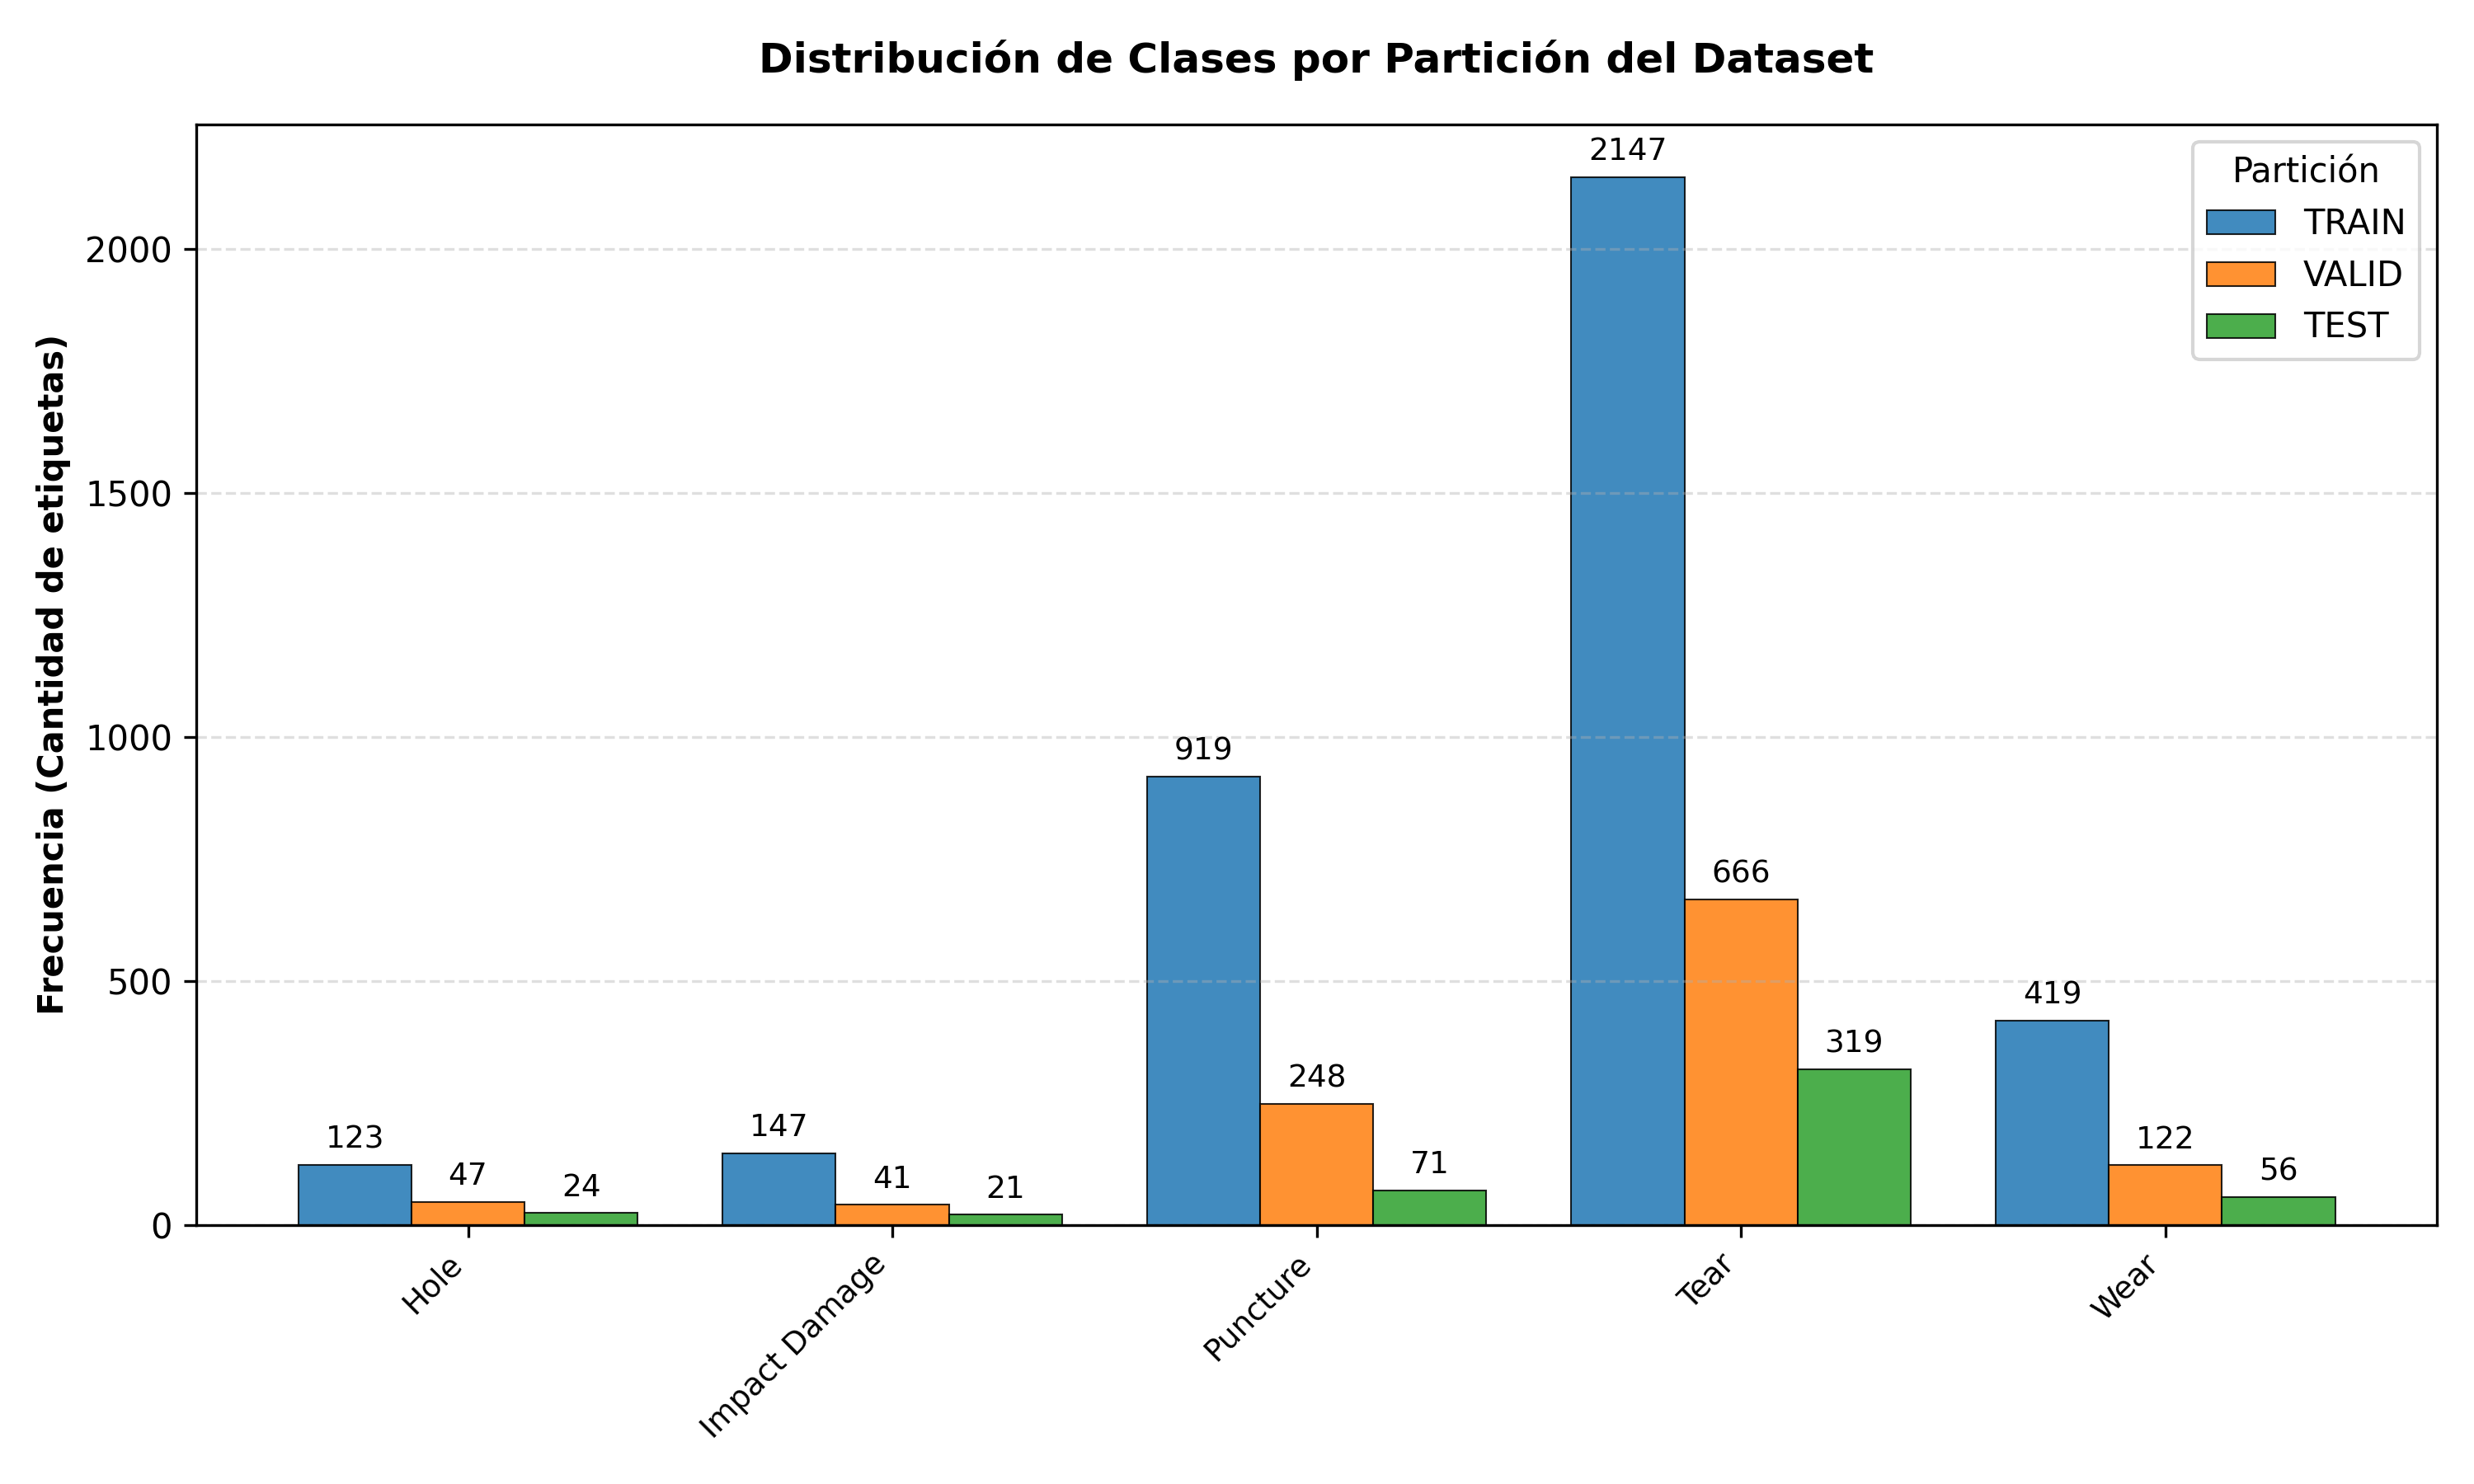
\includegraphics[width=0.8\textwidth]{img/4-Resultados_Discusion/Dataset/class_distribution.png}
    \caption{Distribución de frecuencia de las clases de fallas a través de las particiones del conjunto de datos.}
    \label{fig:4.1-dataset_classes}
\end{figure}

\begin{figure}[H]
    \centering
    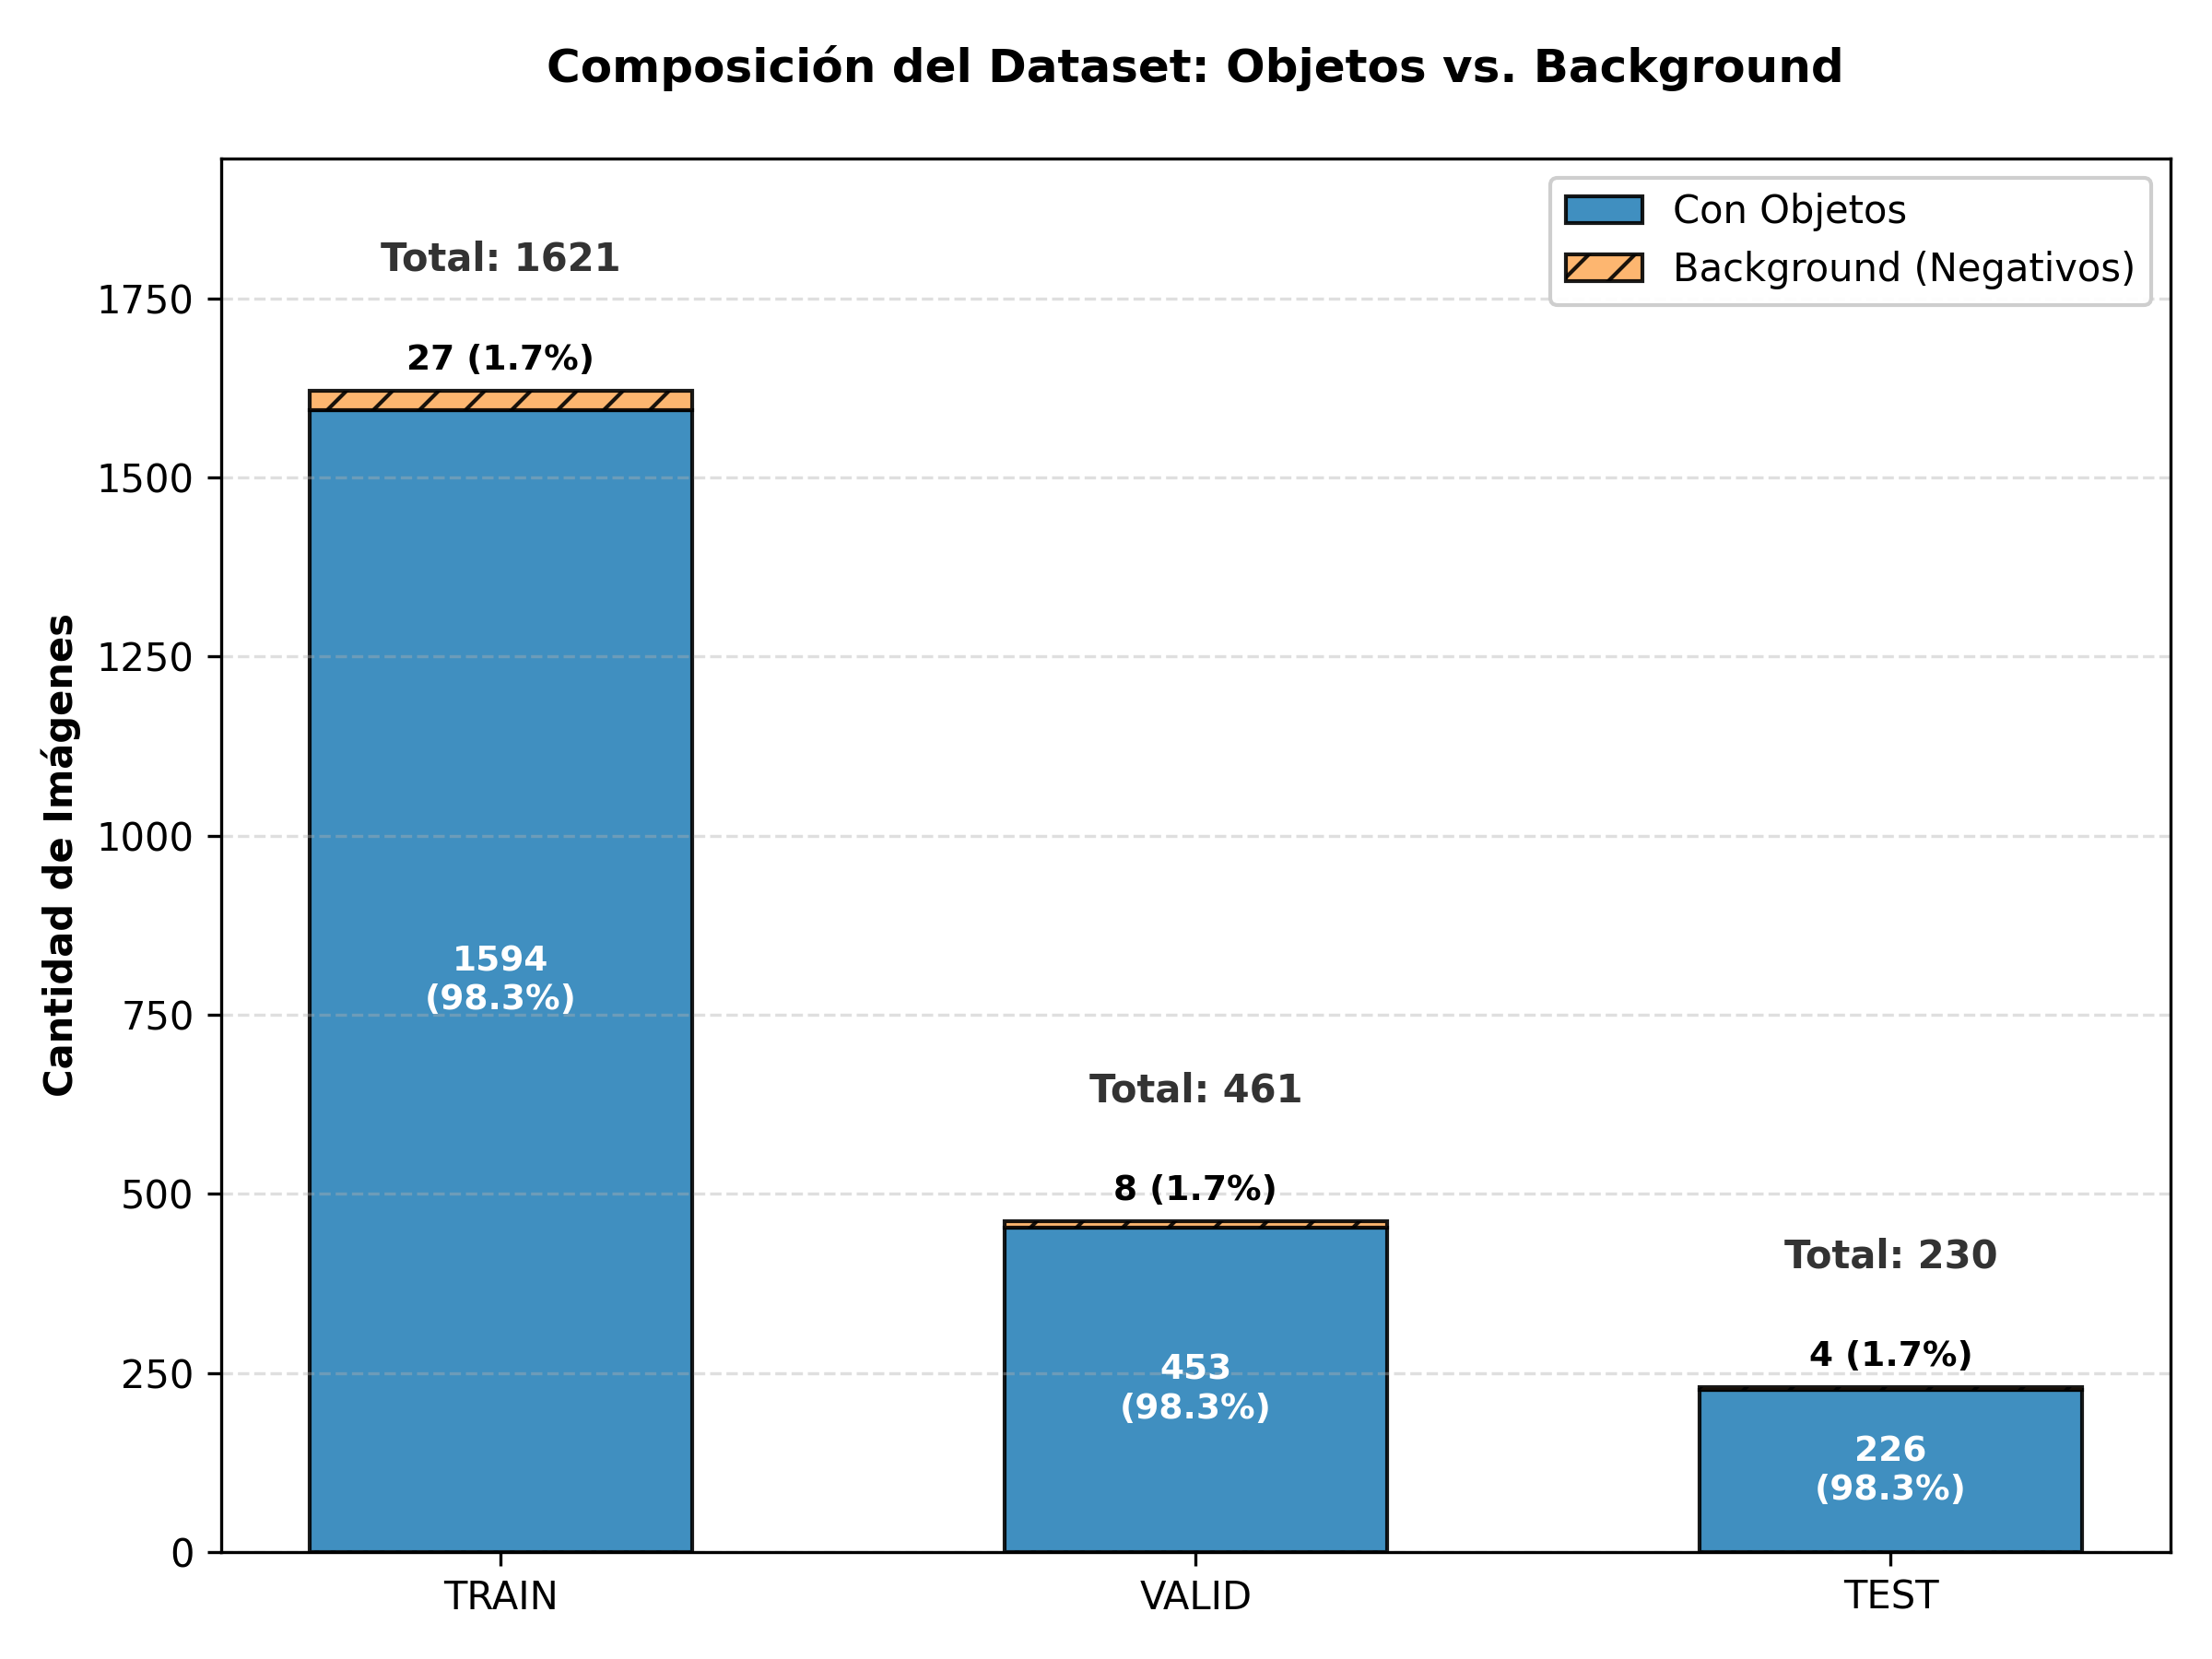
\includegraphics[width=0.8\textwidth]{img/4-Resultados_Discusion/Dataset/split_composition.png}
    \caption{Composición detallada de las particiones del conjunto de datos, diferenciando entre imágenes con objetos y casos de fondo.}
    \label{fig:4.1-dataset_split_compo}
\end{figure}




%%%%%%%%%%%%%%%%%%%%%%%%%%%%%%%%%%%%%%%%%%%%%%%%%%%%%%%%%%%%%%%%%%%%%%%%%%%%%%%%%%%%%%%%%%%%%%%%%%%%%%%%%%%%%%%%%%%%%%%%%%%%%%%%%%%%%%%%%%%%%%%%%%%%%%%%%%%%%%%%%%%%%%%%%%%%%%%%%%%%%%%%%%%%%%%%%%%%%%%%%%%%%%%%%%%%%%%%%%%%%%%%%%%%%%%%%%%%%%%%%%%%%%%%%%%%%%%%%%%%%%%%%%%%%%%%%%%%%%%%%%%%%%%%%%%%%%

\clearpage
\section{Métricas modelos de una sola etapa}


%%%%%%%%%%%%%%%%%%%%%%%%%%%%%%%%%%%%%%%%%%%%%%%%%%%%%%%%%%%%%%%%%%%%%%%%%%%%%%%%%%%%%%%%%%%%%%%%%%
\subsection{YOLOv5}

\par En esta subsección, se exponen y discuten los resultados obtenidos tras el entrenamiento del modelo \textbf{YOLOv5} en su variante \textbf{s} (small), utilizando la configuración de hiperparámetros detallada previamente en la Tabla \ref{tab:3.3-hiperparametros-yolov5}.

% Si alcanzamos, variante x (más pesada), para ver extremos entre velocidad-precision.

%%%%%%%%%%%%%%%%%%%%%%%%%%%%%%%%%%%%%%%%%%%%%%%%%%%%%
\subsubsection{Curva de pérdida vs época por componentes}


%%%%%%%%%%%%%%%%%%%%%%%%%%%%%%%%%%%%%%%%%%%%%%%%%%
\subsubsection{Curva de pérdida vs época promedio}

%%%%%%%%%%%%%%%%%%%%%%%%%%%%%%%%%%%%%%%%%%%%%%%%%%
\subsubsection{Precision y Recall}


%%%%%%%%%%%%%%%%%%%%%%%%%%%%%%%%%%%%%%%%%%%%%%%%%%
\subsubsection{F1-Score}

%%%%%%%%%%%%%%%%%%%%%%%%%%%%%%%%%%%%%%%%%%%%%%%%%%
\subsubsection{Precisión Promedio Media (mAP)}


%%%%%%%%%%%%%%%%%%%%%%%%%%%%%%%%%%%%%%%%%%%%%%%%%%
\subsubsection{Distribución de IoU}

%%%%%%%%%%%%%%%%%%%%%%%%%%%%%%%%%%%%%%%%%%%%%%%%%%
\subsubsection{Matriz de Confusión}



\clearpage
%%%%%%%%%%%%%%%%%%%%%%%%%%%%%%%%%%%%%%%%%%%%%%%%%%%%%%%%%%%%%%%%%%%%%%%%%%%%%%%%%%%%%%%%%%%%%%%%%%%%%%%%%%%%%%%%%%%%%%%%%%%%%%%%%%%%%%%%%%%%%%%%%%%%%%%%%%%%%%%%%%%%%%%%%%%%%%%%%%%%%%%%%%%%%%%%%%%%%%%%%%%%
\subsection{SSD}

\par A continuación, se presentan los resultados obtenidos para el modelo \textbf{SSD300}. Este modelo fue entrenado utilizando una resolución de entrada de $300\times300$ píxeles y la configuración de hiperparámetros detallada en la Tabla \ref{tab:3.4-hiperparametros-ssd}. El análisis se enfoca en evaluar la estabilidad del entrenamiento y la capacidad del detector para operar con mapas de características de menor resolución espacial en comparación con YOLOv5.

%%%%%%%%%%%%%%%%%%%%%%%%%%%%%%%%%%%%%%%%%%%%%%%%%%
\subsubsection{Curva de pérdida vs época específicas}


%%%%%%%%%%%%%%%%%%%%%%%%%%%%%%%%%%%%%%%%%%%%%%%%%%
\subsubsection{Curva de pérdida vs época promedio}

%%%%%%%%%%%%%%%%%%%%%%%%%%%%%%%%%%%%%%%%%%%%%%%%%%
\subsubsection{Precision y Recall}


%%%%%%%%%%%%%%%%%%%%%%%%%%%%%%%%%%%%%%%%%%%%%%%%%%
\subsubsection{F1-Score}


%%%%%%%%%%%%%%%%%%%%%%%%%%%%%%%%%%%%%%%%%%%%%%%%%%
\subsubsection{Precisión Promedio Media (mAP)}



%%%%%%%%%%%%%%%%%%%%%%%%%%%%%%%%%%%%%%%%%%%%%%%%%%
\subsubsection{Distribución de IoU}







%%%%%%%%%%%%%%%%%%%%%%%%%%%%%%%%%%%%%%%%%%%%%%%%%%
\subsubsection{Matriz de Confusión}

\clearpage

\chapter{Conclusiones}

En el presente trabajo de memoria se cumplió con el objetivo general de implementar y evaluar algoritmos de detección de objetos, basados en inteligencia artificial, para la identificación automática de fallas en correas transportadoras. Asimismo, los objetivos específicos y alcances propuestos fueron logrados con éxito. Se implementaron y evaluaron dos arquitecturas convolucionales asociadas a modelos de detección de objetos de una sola etapa (YOLOv5 y SSD) junto con modelos basados en mecanismos de atención global con arquitectura (\textit{transformer}) (DETR y DINO). Todo el proceso de entrenamiento, validación y prueba se realizó utilizando una base de datos pública debidamente estructurada, considerando cinco clases de falla y un esquema estandarizado que permitió una evaluación cuantitativa ordenada y precisa.\\


Respecto a los resultados y discusiones, la variante \textit{small} (s) de YOLOv5 se consolidó como el modelo superior al maximizar la eficiencia, mientras que SSD512 obtuvo el rendimiento más deficiente. El mayor desafío recayó en la detección deficiente de la clase perforación (\textit{Puncture}); no obstante, DINO-R50-4scale demostró ligera superioridad prediciendo este defecto gracias a su atención global y su mecanismo mejorado de eliminación de ruido contrastivo. \\

El desempeño de las arquitecturas \textit{Transformers} se vio penalizado por la escala de los datos, la brecha de dominio y las restricciones físicas. Su extremo consumo de memoria forzó a reducir los tamaño de lote, ralentizando la convergencia de los gradientes y aumentando los tiempos de entrenamiento. Al mantener un régimen estandarizado sin optimización profunda de hiperparámetros, los detectores convolucionales \textit{One-Stage} se ratifican como la alternativa de mayor viabilidad práctica e industrial en la actualidad. \\

Como trabajo futuro se propone: una optimización de hiperparámetros para cada modelo; la ejecución de entrenamientos en escritorios fijos dedicado, en vez de equipos portátiles; y la implementación de arquitecturas híbridas (como RT-DETR o DELO), orientadas a fusionar la eficiencia de extracción local de las CNN con el mecanismo de atención global de los \textit{Transformers}.
\bibliography{library}
\chapter{Anexos}

\section{Tablas de Hiperparámetros}

\begin{table}[H]
    \centering
    \caption{Hiperparámetros principales seleccionados para el entrenamiento de YOLOv5.}
    \begin{tabular}{|c|c|c|}
        \hline
        \textbf{Hiperparámetro} & \textbf{Valor seleccionado} & \textbf{Nombre} \\
        \hline 
        $variant$ & s & Variante del modelo \\
        \hline
        $img\_size$ & 640 & Tamaño imagen de entrada \\
        \hline
        $optimizer$ & SGD & Optimizador de entrenamiento \\
        \hline
        $lr0$ & 0.01 & Tasa de aprendizaje inicial \\
        \hline
        $lrf$ & 0.01 & Factor de tasa final \\
        \hline
        $momentum$ & 0.937 & Momento del optimizador \\
        \hline
        $weight\_decay$ & 0.0005 & Regularización $L_2$ \\
        \hline
        $batch\_size$ & 8 & Tamaño de lote de entrenamiento \\
        \hline
        $warmup\_epochs$ & 3.0 & Épocas de calentamiento \\
        \hline
        $warmup\_momentum$ & 0.8 & Momento en calentamiento \\
        \hline
        $warmup\_bias\_lr$ & 0.1 & Tasa de aprendizaje sesgos calentamiento \\
        \hline
        $box$ & 0.05 & Peso pérdida de cajas \\
        \hline
        $cls$ & 0.5 & Peso pérdida de clasificación \\
        \hline
        $obj$ & 1.0 & Peso pérdida de objeto \\
        \hline
        $iou\_t$ & 0.2 & Umbral IoU para anclas \\
        \hline
        $anchor\_t$ & 4.0 & Umbral de ajuste de anclas \\
        \hline
        $hsv\_h$ & 0.015 & Aumentación en tono HSV \\
        \hline
        $hsv\_s$ & 0.7 & Aumentación en saturación HSV \\
        \hline
        $hsv\_v$ & 0.4 & Aumentación en valor HSV \\
        \hline
        $translate$ & 0.1 & Traslación geométrica \\
        \hline
        $scale$ & 0.5 & Escalamiento aleatorio \\
        \hline
        $fliplr$ & 0.5 & Volteo horizontal \\
        \hline
        $mosaic$ & 1.0 & Aumentación tipo mosaico \\
        \hline
    \end{tabular}
    \label{tab:3.3-hiperparametros-yolov5}
\end{table}


\begin{table}[H]
    \centering
    \caption{Hiperparámetros principales seleccionados para el entrenamiento de SSD300.}
    \begin{tabular}{|c|c|c|}
        \hline
        \textbf{Hiperparámetro} & \textbf{Valor seleccionado} & \textbf{Nombre} \\
        \hline
        $min\_dim$ & 300 & Tamaño de entrada ($300\times300$) \\
        \hline
        $mean$ & (104, 117, 123) & Media de normalización \\
        \hline
        $optimizer$ & SGD & Optimizador \\
        \hline
        $lr$ & $1\times10^{-3}$ & Tasa de aprendizaje inicial \\
        \hline
        $\gamma$ & 0.1 & Factor de decaimiento de $lr$ \\
        \hline
        $lr\_steps$ & $\{80k, 100k, 120k\}$ & Iteraciones de ajuste de $lr$ \\
        \hline
        $momentum$ & 0.9 & Momento del optimizador \\
        \hline
        $weight\_decay$ & $5\times10^{-4}$ & Regularización $L_2$ \\
        \hline
        $batch\_size$ & 16 & Tamaño de lote de entrenamiento \\
        \hline
        $overlap\_thresh$ & 0.5 & Umbral IoU para \textit{matching} positivo \\
        \hline
        $neg\_pos\_ratio$ & 3 & Relación negativos:positivos \\
        \hline
        $neg\_overlap$ & 0.5 & Umbral IoU para negativos \\
        \hline
        $conf\_thresh$ & 0.01 & Umbral mínimo de confianza \\
        \hline
        $nms\_thresh$ & 0.45 & Umbral IoU para NMS \\
        \hline
        $brightness\_\delta$ & 32 & Rango de brillo aleatorio \\
        \hline
        $contrast\_range$ & [0.5, 1.5] & Rango de contraste aleatorio \\
        \hline
        $saturation\_range$ & [0.5, 1.5] & Rango de saturación aleatoria \\
        \hline
        $hue\_\delta$ & 18 & Variación máxima de tono \\
        \hline
        $random\_mirror$ & 0.5 & Probabilidad de volteo horizontal \\
        \hline
    \end{tabular}
    \label{tab:3.4-hiperparametros-ssd}
\end{table}



% FIN DEL DOCUMENTO
\end{document}
